% Options for packages loaded elsewhere
\PassOptionsToPackage{unicode}{hyperref}
\PassOptionsToPackage{hyphens}{url}
%
\documentclass[
]{article}
\usepackage{lmodern}
\usepackage{amssymb,amsmath}
\usepackage{ifxetex,ifluatex}
\ifnum 0\ifxetex 1\fi\ifluatex 1\fi=0 % if pdftex
  \usepackage[T1]{fontenc}
  \usepackage[utf8]{inputenc}
  \usepackage{textcomp} % provide euro and other symbols
\else % if luatex or xetex
  \usepackage{unicode-math}
  \defaultfontfeatures{Scale=MatchLowercase}
  \defaultfontfeatures[\rmfamily]{Ligatures=TeX,Scale=1}
\fi
% Use upquote if available, for straight quotes in verbatim environments
\IfFileExists{upquote.sty}{\usepackage{upquote}}{}
\IfFileExists{microtype.sty}{% use microtype if available
  \usepackage[]{microtype}
  \UseMicrotypeSet[protrusion]{basicmath} % disable protrusion for tt fonts
}{}
\makeatletter
\@ifundefined{KOMAClassName}{% if non-KOMA class
  \IfFileExists{parskip.sty}{%
    \usepackage{parskip}
  }{% else
    \setlength{\parindent}{0pt}
    \setlength{\parskip}{6pt plus 2pt minus 1pt}}
}{% if KOMA class
  \KOMAoptions{parskip=half}}
\makeatother
\usepackage{xcolor}
\IfFileExists{xurl.sty}{\usepackage{xurl}}{} % add URL line breaks if available
\IfFileExists{bookmark.sty}{\usepackage{bookmark}}{\usepackage{hyperref}}
\hypersetup{
  pdftitle={00-Data-Processing-Example},
  hidelinks,
  pdfcreator={LaTeX via pandoc}}
\urlstyle{same} % disable monospaced font for URLs
\usepackage[margin=1in]{geometry}
\usepackage{color}
\usepackage{fancyvrb}
\newcommand{\VerbBar}{|}
\newcommand{\VERB}{\Verb[commandchars=\\\{\}]}
\DefineVerbatimEnvironment{Highlighting}{Verbatim}{commandchars=\\\{\}}
% Add ',fontsize=\small' for more characters per line
\usepackage{framed}
\definecolor{shadecolor}{RGB}{248,248,248}
\newenvironment{Shaded}{\begin{snugshade}}{\end{snugshade}}
\newcommand{\AlertTok}[1]{\textcolor[rgb]{0.94,0.16,0.16}{#1}}
\newcommand{\AnnotationTok}[1]{\textcolor[rgb]{0.56,0.35,0.01}{\textbf{\textit{#1}}}}
\newcommand{\AttributeTok}[1]{\textcolor[rgb]{0.77,0.63,0.00}{#1}}
\newcommand{\BaseNTok}[1]{\textcolor[rgb]{0.00,0.00,0.81}{#1}}
\newcommand{\BuiltInTok}[1]{#1}
\newcommand{\CharTok}[1]{\textcolor[rgb]{0.31,0.60,0.02}{#1}}
\newcommand{\CommentTok}[1]{\textcolor[rgb]{0.56,0.35,0.01}{\textit{#1}}}
\newcommand{\CommentVarTok}[1]{\textcolor[rgb]{0.56,0.35,0.01}{\textbf{\textit{#1}}}}
\newcommand{\ConstantTok}[1]{\textcolor[rgb]{0.00,0.00,0.00}{#1}}
\newcommand{\ControlFlowTok}[1]{\textcolor[rgb]{0.13,0.29,0.53}{\textbf{#1}}}
\newcommand{\DataTypeTok}[1]{\textcolor[rgb]{0.13,0.29,0.53}{#1}}
\newcommand{\DecValTok}[1]{\textcolor[rgb]{0.00,0.00,0.81}{#1}}
\newcommand{\DocumentationTok}[1]{\textcolor[rgb]{0.56,0.35,0.01}{\textbf{\textit{#1}}}}
\newcommand{\ErrorTok}[1]{\textcolor[rgb]{0.64,0.00,0.00}{\textbf{#1}}}
\newcommand{\ExtensionTok}[1]{#1}
\newcommand{\FloatTok}[1]{\textcolor[rgb]{0.00,0.00,0.81}{#1}}
\newcommand{\FunctionTok}[1]{\textcolor[rgb]{0.00,0.00,0.00}{#1}}
\newcommand{\ImportTok}[1]{#1}
\newcommand{\InformationTok}[1]{\textcolor[rgb]{0.56,0.35,0.01}{\textbf{\textit{#1}}}}
\newcommand{\KeywordTok}[1]{\textcolor[rgb]{0.13,0.29,0.53}{\textbf{#1}}}
\newcommand{\NormalTok}[1]{#1}
\newcommand{\OperatorTok}[1]{\textcolor[rgb]{0.81,0.36,0.00}{\textbf{#1}}}
\newcommand{\OtherTok}[1]{\textcolor[rgb]{0.56,0.35,0.01}{#1}}
\newcommand{\PreprocessorTok}[1]{\textcolor[rgb]{0.56,0.35,0.01}{\textit{#1}}}
\newcommand{\RegionMarkerTok}[1]{#1}
\newcommand{\SpecialCharTok}[1]{\textcolor[rgb]{0.00,0.00,0.00}{#1}}
\newcommand{\SpecialStringTok}[1]{\textcolor[rgb]{0.31,0.60,0.02}{#1}}
\newcommand{\StringTok}[1]{\textcolor[rgb]{0.31,0.60,0.02}{#1}}
\newcommand{\VariableTok}[1]{\textcolor[rgb]{0.00,0.00,0.00}{#1}}
\newcommand{\VerbatimStringTok}[1]{\textcolor[rgb]{0.31,0.60,0.02}{#1}}
\newcommand{\WarningTok}[1]{\textcolor[rgb]{0.56,0.35,0.01}{\textbf{\textit{#1}}}}
\usepackage{graphicx,grffile}
\makeatletter
\def\maxwidth{\ifdim\Gin@nat@width>\linewidth\linewidth\else\Gin@nat@width\fi}
\def\maxheight{\ifdim\Gin@nat@height>\textheight\textheight\else\Gin@nat@height\fi}
\makeatother
% Scale images if necessary, so that they will not overflow the page
% margins by default, and it is still possible to overwrite the defaults
% using explicit options in \includegraphics[width, height, ...]{}
\setkeys{Gin}{width=\maxwidth,height=\maxheight,keepaspectratio}
% Set default figure placement to htbp
\makeatletter
\def\fps@figure{htbp}
\makeatother
\setlength{\emergencystretch}{3em} % prevent overfull lines
\providecommand{\tightlist}{%
  \setlength{\itemsep}{0pt}\setlength{\parskip}{0pt}}
\setcounter{secnumdepth}{-\maxdimen} % remove section numbering

\title{00-Data-Processing-Example}
\author{}
\date{\vspace{-2.5em}}

\begin{document}
\maketitle

\hypertarget{introduction}{%
\subsection{Introduction}\label{introduction}}

In this notebook we create some examples of processing the data for the
analysis of accessibility to Hamilton Bike share docking stations.
Particularly, we're interested in spatial interpolation of the
population for small areas.

Data used in this notebook was retrieved from two sources: Open Hamilton
and the 2016 Canadian Census. Open Hamilton is an online repository of
data from the City of Hamilton. The following datasets were retrieved:

\hypertarget{provenance-of-data}{%
\subsection{Provenance of data}\label{provenance-of-data}}

\hypertarget{sobi-hub}{%
\subsubsection{SoBi Hub}\label{sobi-hub}}

The dataset was last updated on \emph{November 9, 2020} and was
downloaded for this project on \emph{November 10, 2020}. This dataset
contains the following attributes that are of interest to this research:
location of hubs (address, longitude, and latitude) and the number of
racks available at each hub. The dataset also includes the number of
bicycles available at each hub, but since this changes daily, this
information is not useful for our purposes. The maximum number of
bicycles that a hub \emph{could} have (i.e., the baseline) available is
important for calculating accessibility in a given area.

We can also retrieve the data weekly over a certain period, for example
4 weeks, to calculate the average number of bicycles that are at each
hub. Variations in the number of bicycles could also be informative. For
instance, some hubs may systematically have more or less bicycles than
others (i.e., excess of supply around the University campus).

\hypertarget{sobi-service-area}{%
\subsubsection{SoBi Service Area}\label{sobi-service-area}}

The dataset was last updated on \emph{November 9, 2020} and was
downloaded for this project on \emph{November 10, 2020}. Hamilton's bike
share program is available only in the lower city from Dundas to Ottawa
Street North. There is one isolated hub beyond this service area at Van
Wagner's Beach for tourism purposes.

\hypertarget{golf-courses}{%
\subsubsection{Golf Courses}\label{golf-courses}}

The dataset was last updated on \emph{November 1, 2020} and was
downloaded for this project on \emph{November 10, 2020}. This dataset
contains the location of City and privately owned golf courses in
Hamilton.

\hypertarget{parks}{%
\subsubsection{Parks}\label{parks}}

The dataset was last updated on \emph{November 8, 2020} and was
downloaded for this project on \emph{November 10, 2020}. This dataset
contains the location of parks and other green spaces in Hamilton.

\hypertarget{large-employment-areas}{%
\subsubsection{Large Employment Areas}\label{large-employment-areas}}

The dataset contains Employment Land boundaries in Hamilton and was last
updated on \emph{November 12, 2020}. It was downloaded for this project
on \emph{November 13, 2020}. This dataset contains the location of large
business parks and industrial lands in Hamilton.

\hypertarget{municipal-parking-lots}{%
\subsubsection{Municipal Parking Lots}\label{municipal-parking-lots}}

The dataset contains the location of municipal car parks in Hamilton and
was last updated on \emph{November 9, 2020}. It was downloaded for this
project on \emph{November 13, 2020}.

\hypertarget{cemeteries}{%
\subsubsection{Cemeteries}\label{cemeteries}}

The dataset contains the location of cemeteries in Hamilton. It was
downloaded for this project on \emph{November 13, 2020}.

\hypertarget{environmentally-sensitive-areas}{%
\subsubsection{Environmentally Sensitive
Areas}\label{environmentally-sensitive-areas}}

The dataset contains the location of Environmentally Sensitive Areas
(ESAs) in Hamilton. ESAs are either land or water areas containing
natural features or significant ecological functions in Hamilton. The
data were downloaded on \emph{November 13, 2020}.

\hypertarget{street-centreline}{%
\subsubsection{Street Centreline}\label{street-centreline}}

The dataset contains the street network in Hamilton. Data attributes
include road classification so highways can be extracted. The dataset
was last updated on \emph{November 15, 2020} and downloaded on
\emph{November 16, 2020}.

\hypertarget{educational-institutions}{%
\subsubsection{Educational
Institutions}\label{educational-institutions}}

The dataset contains the location of all educational institutions and
schools in Hamilton. The dataset was last updated on \emph{November 15,
2020} and downloaded on \emph{November 16, 2020}.

\hypertarget{places-of-workshop}{%
\subsubsection{Places of Workshop}\label{places-of-workshop}}

The dataset contains the location of buildings used for religious
congregations in Hamilton. The dataset was last updated on
\emph{November 15, 2020} and downloaded on \emph{November 16, 2020}.

\hypertarget{municipal-service-centres}{%
\subsubsection{Municipal Service
Centres}\label{municipal-service-centres}}

The dataset contains the location of all municipal service centres in
Hamilton. This includes Hamilton City Hall. The dataset was last updated
on \emph{November 11, 2020} and downloaded on \emph{November 16, 2020}.

\hypertarget{recreation-and-community-centres}{%
\subsubsection{Recreation and Community
Centres}\label{recreation-and-community-centres}}

The dataset contains the location of all recreation and community
centres in Hamilton. This includes Hamilton City Hall. The dataset was
last updated on \emph{November 15, 2020} and downloaded on
\emph{November 16, 2020}.

\hypertarget{arenas}{%
\subsubsection{Arenas}\label{arenas}}

The dataset contains the location of all indoor arenas in Hamilton. This
includes Hamilton City Hall. The dataset was last updated on
\emph{November 12, 2020} and downloaded on \emph{November 16, 2020}.

\hypertarget{ems-stations}{%
\subsubsection{EMS Stations}\label{ems-stations}}

The dataset contains the location of all Emergency Management Services
(EMS) Ambulance stations in Hamilton. This includes Hamilton City Hall.
The dataset was last updated on \emph{November 11, 2020} and downloaded
on \emph{November 16, 2020}.

\hypertarget{fire-stations}{%
\subsubsection{Fire Stations}\label{fire-stations}}

The dataset contains the location of all fire stations in Hamilton. This
includes Hamilton City Hall. The dataset was last updated on
\emph{November 15, 2020} and downloaded on \emph{November 16, 2020}.

\hypertarget{police-stations}{%
\subsubsection{Police Stations}\label{police-stations}}

The dataset contains the location of all police stations in Hamilton.
This includes Hamilton City Hall. The dataset was last updated on
\emph{November 13, 2020} and downloaded on \emph{November 16, 2020}.

\hypertarget{hospitals}{%
\subsubsection{Hospitals}\label{hospitals}}

The dataset contains the location of all hospitals in Hamilton. This
includes Hamilton City Hall. The dataset was last updated on \emph{April
2, 2019} and downloaded on \emph{November 16, 2020}.

\hypertarget{preliminaries}{%
\subsection{Preliminaries}\label{preliminaries}}

Clear environment:

\begin{Shaded}
\begin{Highlighting}[]
\KeywordTok{rm}\NormalTok{(}\DataTypeTok{list =} \KeywordTok{ls}\NormalTok{())}
\end{Highlighting}
\end{Shaded}

Load packages used in the notebook:

\begin{Shaded}
\begin{Highlighting}[]
\KeywordTok{library}\NormalTok{(disk.frame)}
\KeywordTok{library}\NormalTok{(pycno)}
\KeywordTok{library}\NormalTok{(readr)}
\KeywordTok{library}\NormalTok{(r5r) }\CommentTok{# the r5r package requires Java Development Kit version 11, which can be downloaded from https://www.oracle.com/java/technologies/javase-jdk11-downloads.html}
\KeywordTok{library}\NormalTok{(sf)}
\KeywordTok{library}\NormalTok{(tidyverse)}
\end{Highlighting}
\end{Shaded}

Define some parameters for \texttt{disk.frame} and \texttt{r5r}:

\begin{Shaded}
\begin{Highlighting}[]
\KeywordTok{setup_disk.frame}\NormalTok{()}
\end{Highlighting}
\end{Shaded}

\begin{verbatim}
## The number of workers available for disk.frame is 4
\end{verbatim}

\begin{Shaded}
\begin{Highlighting}[]
\KeywordTok{options}\NormalTok{(}\DataTypeTok{scipen =} \DecValTok{999}\NormalTok{)}
\KeywordTok{options}\NormalTok{(}\DataTypeTok{java.parameters =} \StringTok{"-Xmx6G"}\NormalTok{)}
\KeywordTok{options}\NormalTok{(}\DataTypeTok{future.globals.maxSize =} \OtherTok{Inf}\NormalTok{)}
\end{Highlighting}
\end{Shaded}

\hypertarget{read-data}{%
\subsubsection{Read data}\label{read-data}}

Load data files:

\begin{Shaded}
\begin{Highlighting}[]
\KeywordTok{load}\NormalTok{(}\StringTok{"hamilton_cma.RData"}\NormalTok{)}
\KeywordTok{load}\NormalTok{(}\StringTok{"hamilton_da_2016.RData"}\NormalTok{)}
\end{Highlighting}
\end{Shaded}

These two data files are simple features with the dissemination areas
according to the 2016 Census, and the boundary of Hamilton CMA.

\begin{Shaded}
\begin{Highlighting}[]
\KeywordTok{ggplot}\NormalTok{() }\OperatorTok{+}
\StringTok{  }\KeywordTok{geom_sf}\NormalTok{(}\DataTypeTok{data =}\NormalTok{ hamilton_cma)}
\end{Highlighting}
\end{Shaded}

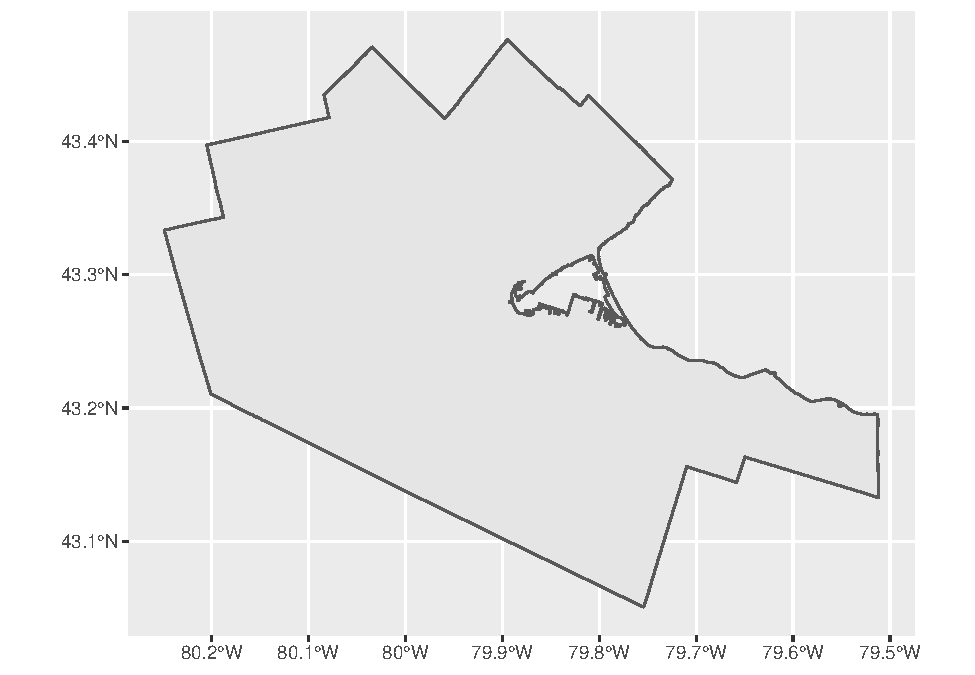
\includegraphics{00-Data-Processing-Example_files/figure-latex/unnamed-chunk-5-1.pdf}

\begin{Shaded}
\begin{Highlighting}[]
\KeywordTok{ggplot}\NormalTok{() }\OperatorTok{+}
\StringTok{  }\KeywordTok{geom_sf}\NormalTok{(}\DataTypeTok{data =}\NormalTok{ hamilton_da_}\DecValTok{2016}\NormalTok{)}
\end{Highlighting}
\end{Shaded}

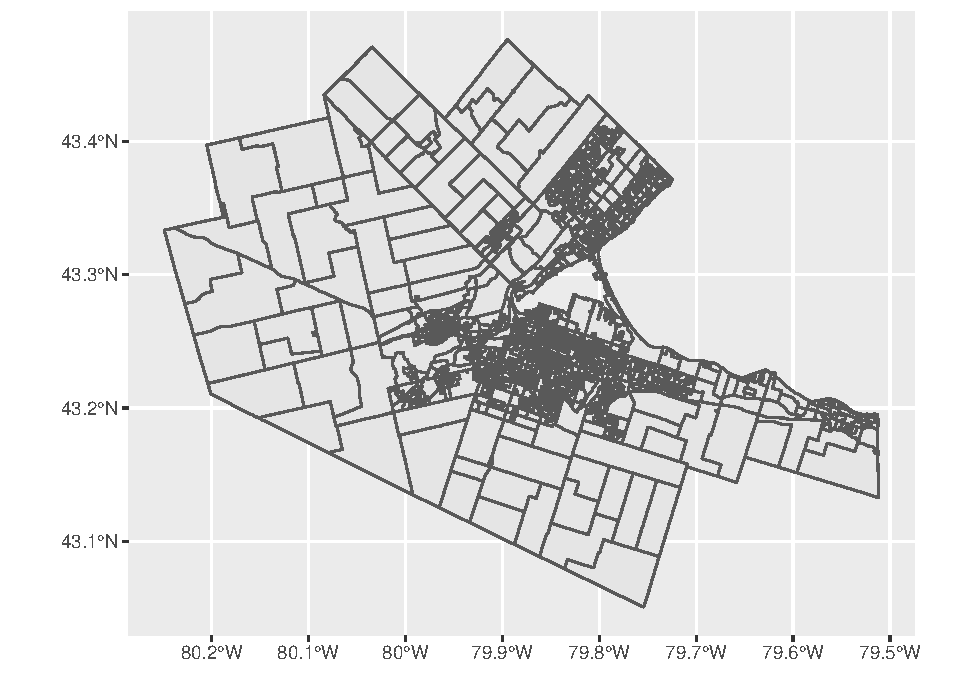
\includegraphics{00-Data-Processing-Example_files/figure-latex/unnamed-chunk-6-1.pdf}

Read Sobi service area:

\begin{Shaded}
\begin{Highlighting}[]
\NormalTok{sobi_service <-}\StringTok{ }\KeywordTok{st_read}\NormalTok{(}\StringTok{"SoBi_Service_Areas.shp"}\NormalTok{)}
\end{Highlighting}
\end{Shaded}

\begin{verbatim}
## Reading layer `SoBi_Service_Areas' from data source `C:\Users\desjae\Documents\GitHub\Accessibility-Sobi-Hamilton\examples\SoBi_Service_Areas.shp' using driver `ESRI Shapefile'
## Simple feature collection with 2 features and 3 fields
## geometry type:  POLYGON
## dimension:      XY
## bbox:           xmin: 583329.4 ymin: 4787385 xmax: 600145.7 ymax: 4793252
## projected CRS:  NAD83 / UTM zone 17N
\end{verbatim}

Plot service areas:

\begin{Shaded}
\begin{Highlighting}[]
\KeywordTok{ggplot}\NormalTok{() }\OperatorTok{+}
\StringTok{  }\KeywordTok{geom_sf}\NormalTok{(}\DataTypeTok{data =}\NormalTok{ sobi_service,}
          \KeywordTok{aes}\NormalTok{(}\DataTypeTok{fill =}\NormalTok{ AREA_NAME))}
\end{Highlighting}
\end{Shaded}

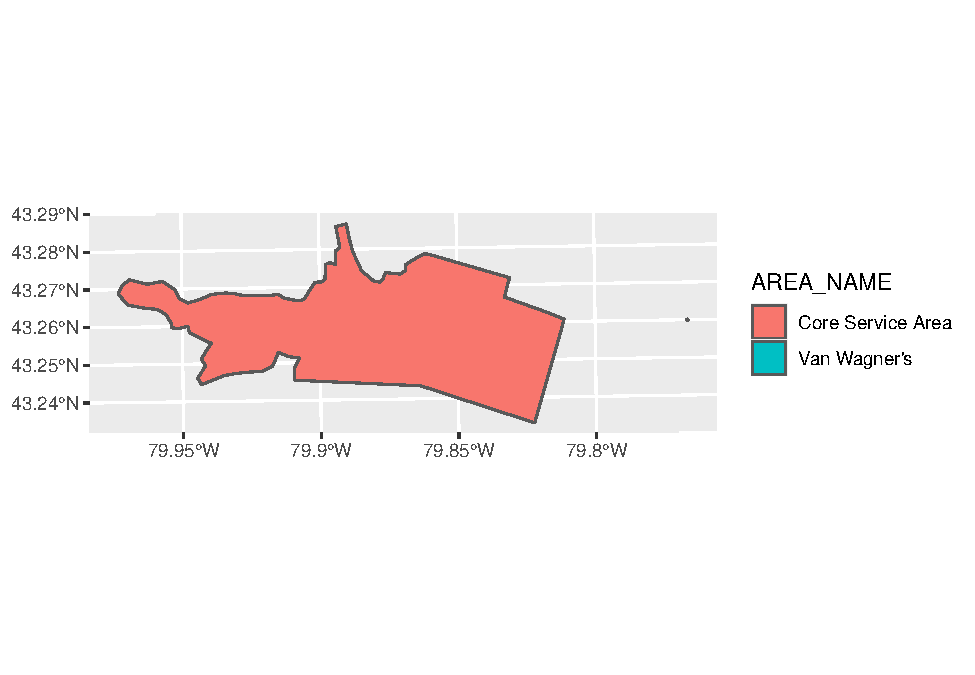
\includegraphics{00-Data-Processing-Example_files/figure-latex/unnamed-chunk-8-1.pdf}

There is a Core Service Area and a much smaller service area at Van
Wagner's. This is a location at the beach with service for beach goers.
We will remove this area from further analysis:

\begin{Shaded}
\begin{Highlighting}[]
\NormalTok{sobi_service <-}\StringTok{ }\NormalTok{sobi_service }\OperatorTok
\StringTok{  }\NormalTok{dplyr}\OperatorTok{::}\KeywordTok{filter}\NormalTok{(AREA_NAME }\OperatorTok{==}\StringTok{ "Core Service Area"}\NormalTok{)}
\end{Highlighting}
\end{Shaded}

Bounding box of population in serviced areas:

\begin{Shaded}
\begin{Highlighting}[]
\NormalTok{bounding_box <-}\StringTok{ }\KeywordTok{st_bbox}\NormalTok{(sobi_service }\OperatorTok
\StringTok{                          }\KeywordTok{st_buffer}\NormalTok{(}\DecValTok{500}\NormalTok{))}
\end{Highlighting}
\end{Shaded}

Plot:

\begin{Shaded}
\begin{Highlighting}[]
\KeywordTok{ggplot}\NormalTok{() }\OperatorTok{+}\StringTok{ }
\StringTok{  }\KeywordTok{geom_sf}\NormalTok{(}\DataTypeTok{data =}\NormalTok{ hamilton_da_}\DecValTok{2016}\NormalTok{,}
          \DataTypeTok{fill =} \OtherTok{NA}\NormalTok{,}
          \DataTypeTok{color =} \StringTok{"lightgray"}\NormalTok{) }\OperatorTok{+}\StringTok{ }
\StringTok{  }\KeywordTok{geom_sf}\NormalTok{(}\DataTypeTok{data =}\NormalTok{ sobi_service,}
          \DataTypeTok{fill =} \OtherTok{NA}\NormalTok{) }\OperatorTok{+}
\StringTok{  }\KeywordTok{geom_sf}\NormalTok{(}\DataTypeTok{data =} \KeywordTok{st_as_sfc}\NormalTok{(bounding_box),}
          \DataTypeTok{linetype =} \StringTok{"dashed"}\NormalTok{,}
          \DataTypeTok{fill =} \OtherTok{NA}\NormalTok{)}
\end{Highlighting}
\end{Shaded}

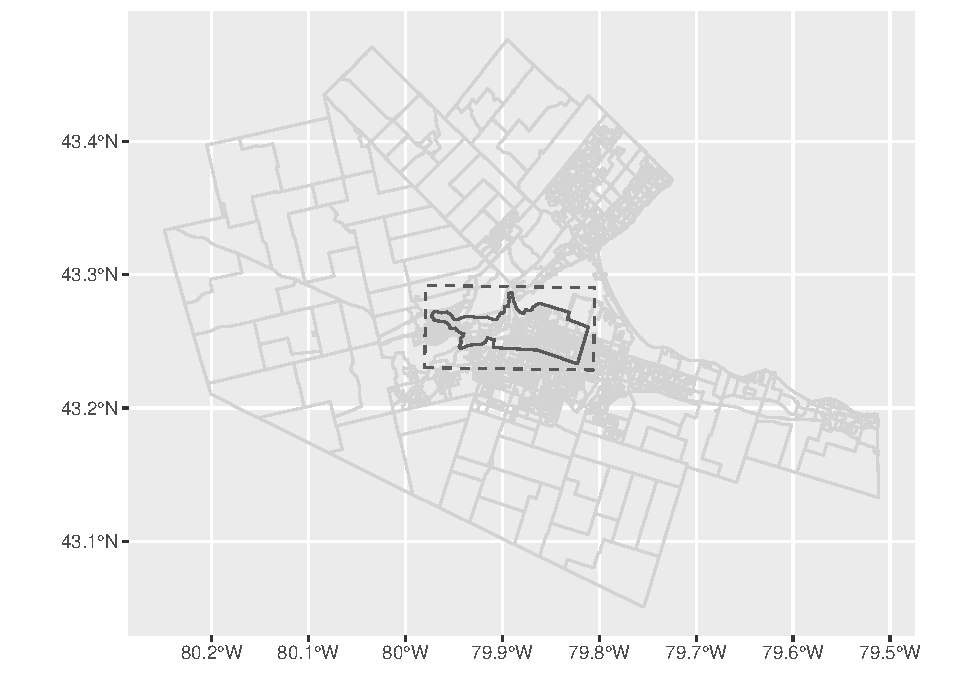
\includegraphics{00-Data-Processing-Example_files/figure-latex/unnamed-chunk-11-1.pdf}

Read parks:

\begin{Shaded}
\begin{Highlighting}[]
\NormalTok{parks <-}\StringTok{ }\KeywordTok{st_read}\NormalTok{(}\StringTok{"Parks.shp"}\NormalTok{)}
\end{Highlighting}
\end{Shaded}

\begin{verbatim}
## Reading layer `Parks' from data source `C:\Users\desjae\Documents\GitHub\Accessibility-Sobi-Hamilton\examples\Parks.shp' using driver `ESRI Shapefile'
## Simple feature collection with 622 features and 7 fields
## geometry type:  MULTIPOLYGON
## dimension:      XY
## bbox:           xmin: 564103.5 ymin: 4774053 xmax: 611193.6 ymax: 4809561
## projected CRS:  NAD83 / UTM zone 17N
\end{verbatim}

Read cemeteries:

\begin{Shaded}
\begin{Highlighting}[]
\NormalTok{cemeteries <-}\StringTok{ }\KeywordTok{st_read}\NormalTok{(}\StringTok{"Cemeteries.shp"}\NormalTok{)}
\end{Highlighting}
\end{Shaded}

\begin{verbatim}
## Reading layer `Cemeteries' from data source `C:\Users\desjae\Documents\GitHub\Accessibility-Sobi-Hamilton\examples\Cemeteries.shp' using driver `ESRI Shapefile'
## Simple feature collection with 31 features and 10 fields
## geometry type:  MULTIPOLYGON
## dimension:      XY
## bbox:           xmin: 567538.9 ymin: 4785183 xmax: 606126.6 ymax: 4794820
## projected CRS:  NAD83 / UTM zone 17N
\end{verbatim}

Read environmentally sensitive areas:

\begin{Shaded}
\begin{Highlighting}[]
\NormalTok{esa <-}\StringTok{ }\KeywordTok{st_read}\NormalTok{(}\StringTok{"Environmentally_Sensitive_Areas_Boundaries.shp"}\NormalTok{)}
\end{Highlighting}
\end{Shaded}

\begin{verbatim}
## Reading layer `Environmentally_Sensitive_Areas_Boundaries' from data source `C:\Users\desjae\Documents\GitHub\Accessibility-Sobi-Hamilton\examples\Environmentally_Sensitive_Areas_Boundaries.shp' using driver `ESRI Shapefile'
## Simple feature collection with 207 features and 9 fields
## geometry type:  POLYGON
## dimension:      XY
## bbox:           xmin: 561664.6 ymin: 4767888 xmax: 611963.3 ymax: 4814265
## projected CRS:  NAD83 / UTM zone 17N
\end{verbatim}

Read golf courses:

\begin{Shaded}
\begin{Highlighting}[]
\NormalTok{golf_courses <-}\StringTok{ }\KeywordTok{st_read}\NormalTok{(}\StringTok{"Golf_Courses.shp"}\NormalTok{)}
\end{Highlighting}
\end{Shaded}

\begin{verbatim}
## Reading layer `Golf_Courses' from data source `C:\Users\desjae\Documents\GitHub\Accessibility-Sobi-Hamilton\examples\Golf_Courses.shp' using driver `ESRI Shapefile'
## Simple feature collection with 27 features and 4 fields
## geometry type:  POLYGON
## dimension:      XY
## bbox:           xmin: 565041.3 ymin: 4771006 xmax: 608445.4 ymax: 4807785
## projected CRS:  NAD83 / UTM zone 17N
\end{verbatim}

Read employment land areas, which include business parks and industrial
lands:

\begin{Shaded}
\begin{Highlighting}[]
\NormalTok{employment_lands <-}\StringTok{ }\KeywordTok{st_read}\NormalTok{(}\StringTok{"Employment_Lands.shp"}\NormalTok{)}
\end{Highlighting}
\end{Shaded}

\begin{verbatim}
## Reading layer `Employment_Lands' from data source `C:\Users\desjae\Documents\GitHub\Accessibility-Sobi-Hamilton\examples\Employment_Lands.shp' using driver `ESRI Shapefile'
## Simple feature collection with 14 features and 5 fields
## geometry type:  MULTIPOLYGON
## dimension:      XY
## bbox:           xmin: 577850.4 ymin: 4778238 xmax: 611498.4 ymax: 4797555
## projected CRS:  NAD83 / UTM zone 17N
\end{verbatim}

Read railways:

\begin{Shaded}
\begin{Highlighting}[]
\NormalTok{railways <-}\StringTok{ }\KeywordTok{st_read}\NormalTok{(}\StringTok{"Railways.shp"}\NormalTok{)}
\end{Highlighting}
\end{Shaded}

\begin{verbatim}
## Reading layer `Railways' from data source `C:\Users\desjae\Documents\GitHub\Accessibility-Sobi-Hamilton\examples\Railways.shp' using driver `ESRI Shapefile'
## Simple feature collection with 1692 features and 4 fields
## geometry type:  MULTILINESTRING
## dimension:      XY
## bbox:           xmin: 563354.6 ymin: 4780233 xmax: 612351 ymax: 4813272
## projected CRS:  NAD83 / UTM zone 17N
\end{verbatim}

Read municipal parking lots:

\begin{Shaded}
\begin{Highlighting}[]
\NormalTok{municipal_parking <-}\StringTok{ }\KeywordTok{st_read}\NormalTok{(}\StringTok{"Municipal_Parking_Lots.shp"}\NormalTok{)}
\end{Highlighting}
\end{Shaded}

\begin{verbatim}
## Reading layer `Municipal_Parking_Lots' from data source `C:\Users\desjae\Documents\GitHub\Accessibility-Sobi-Hamilton\examples\Municipal_Parking_Lots.shp' using driver `ESRI Shapefile'
## Simple feature collection with 62 features and 4 fields
## geometry type:  MULTIPOLYGON
## dimension:      XY
## bbox:           xmin: 583117.5 ymin: 4785525 xmax: 601281.2 ymax: 4798542
## projected CRS:  NAD83 / UTM zone 17N
\end{verbatim}

Read street network:

\begin{Shaded}
\begin{Highlighting}[]
\NormalTok{streets <-}\StringTok{ }\KeywordTok{st_read}\NormalTok{(}\StringTok{"Street_Centreline.shp"}\NormalTok{)}
\end{Highlighting}
\end{Shaded}

\begin{verbatim}
## Reading layer `Street_Centreline' from data source `C:\Users\desjae\Documents\GitHub\Accessibility-Sobi-Hamilton\examples\Street_Centreline.shp' using driver `ESRI Shapefile'
## Simple feature collection with 19396 features and 31 fields
## geometry type:  LINESTRING
## dimension:      XY
## bbox:           xmin: 560789.8 ymin: 4767178 xmax: 611887.1 ymax: 4813706
## projected CRS:  NAD83 / UTM zone 17N
\end{verbatim}

Filter for provincial highways:

\begin{Shaded}
\begin{Highlighting}[]
\NormalTok{streets <-}\StringTok{ }\NormalTok{streets }\OperatorTok\StringTok{ }\NormalTok{dplyr}\OperatorTok{::}\KeywordTok{filter}\NormalTok{(ROAD_CLASS }\OperatorTok{==}\StringTok{ "Provincial Highway"}\NormalTok{)}
\end{Highlighting}
\end{Shaded}

Read educational institutions:

\begin{Shaded}
\begin{Highlighting}[]
\NormalTok{schools <-}\StringTok{ }\KeywordTok{st_read}\NormalTok{(}\StringTok{"Educational_Institutions.shp"}\NormalTok{)}
\end{Highlighting}
\end{Shaded}

\begin{verbatim}
## Reading layer `Educational_Institutions' from data source `C:\Users\desjae\Documents\GitHub\Accessibility-Sobi-Hamilton\examples\Educational_Institutions.shp' using driver `ESRI Shapefile'
## Simple feature collection with 234 features and 14 fields
## geometry type:  POINT
## dimension:      XY
## bbox:           xmin: 564817.6 ymin: 4774480 xmax: 610267.4 ymax: 4806311
## projected CRS:  NAD83 / UTM zone 17N
\end{verbatim}

Read places of worship:

\begin{Shaded}
\begin{Highlighting}[]
\NormalTok{religious_places <-}\StringTok{ }\KeywordTok{st_read}\NormalTok{(}\StringTok{"Places_of_Worship.shp"}\NormalTok{)}
\end{Highlighting}
\end{Shaded}

\begin{verbatim}
## Reading layer `Places_of_Worship' from data source `C:\Users\desjae\Documents\GitHub\Accessibility-Sobi-Hamilton\examples\Places_of_Worship.shp' using driver `ESRI Shapefile'
## Simple feature collection with 356 features and 7 fields
## geometry type:  POINT
## dimension:      XY
## bbox:           xmin: 564564 ymin: 4774769 xmax: 607177.1 ymax: 4809573
## projected CRS:  NAD83 / UTM zone 17N
\end{verbatim}

Read municipal service centres:

\begin{Shaded}
\begin{Highlighting}[]
\NormalTok{service_centres <-}\StringTok{ }\KeywordTok{st_read}\NormalTok{(}\StringTok{"Municipal_Service_Centres.shp"}\NormalTok{)}
\end{Highlighting}
\end{Shaded}

\begin{verbatim}
## Reading layer `Municipal_Service_Centres' from data source `C:\Users\desjae\Documents\GitHub\Accessibility-Sobi-Hamilton\examples\Municipal_Service_Centres.shp' using driver `ESRI Shapefile'
## Simple feature collection with 6 features and 6 fields
## geometry type:  POINT
## dimension:      XY
## bbox:           xmin: 583101.7 ymin: 4775812 xmax: 606290.1 ymax: 4797349
## projected CRS:  NAD83 / UTM zone 17N
\end{verbatim}

Read recreation and centres:

\begin{Shaded}
\begin{Highlighting}[]
\NormalTok{recreation_centres <-}\StringTok{ }\KeywordTok{st_read}\NormalTok{(}\StringTok{"Recreation_and_Community_Centres.shp"}\NormalTok{)}
\end{Highlighting}
\end{Shaded}

\begin{verbatim}
## Reading layer `Recreation_and_Community_Centres' from data source `C:\Users\desjae\Documents\GitHub\Accessibility-Sobi-Hamilton\examples\Recreation_and_Community_Centres.shp' using driver `ESRI Shapefile'
## Simple feature collection with 68 features and 4 fields
## geometry type:  POINT
## dimension:      XY
## bbox:           xmin: 564831.5 ymin: 4775169 xmax: 610016 ymax: 4809482
## projected CRS:  NAD83 / UTM zone 17N
\end{verbatim}

Read arenas:

\begin{Shaded}
\begin{Highlighting}[]
\NormalTok{arenas <-}\StringTok{ }\KeywordTok{st_read}\NormalTok{(}\StringTok{"Arenas.shp"}\NormalTok{)}
\end{Highlighting}
\end{Shaded}

\begin{verbatim}
## Reading layer `Arenas' from data source `C:\Users\desjae\Documents\GitHub\Accessibility-Sobi-Hamilton\examples\Arenas.shp' using driver `ESRI Shapefile'
## Simple feature collection with 25 features and 7 fields
## geometry type:  POINT
## dimension:      XY
## bbox:           xmin: 572082.8 ymin: 4775909 xmax: 605573.3 ymax: 4805382
## projected CRS:  NAD83 / UTM zone 17N
\end{verbatim}

Read EMS stations:

\begin{Shaded}
\begin{Highlighting}[]
\NormalTok{ems <-}\StringTok{ }\KeywordTok{st_read}\NormalTok{(}\StringTok{"EMS_Stations.shp"}\NormalTok{)}
\end{Highlighting}
\end{Shaded}

\begin{verbatim}
## Reading layer `EMS_Stations' from data source `C:\Users\desjae\Documents\GitHub\Accessibility-Sobi-Hamilton\examples\EMS_Stations.shp' using driver `ESRI Shapefile'
## Simple feature collection with 20 features and 7 fields
## geometry type:  POINT
## dimension:      XY
## bbox:           xmin: 569174.6 ymin: 4775023 xmax: 604223.7 ymax: 4798687
## projected CRS:  NAD83 / UTM zone 17N
\end{verbatim}

Read fire stations:

\begin{Shaded}
\begin{Highlighting}[]
\NormalTok{fire <-}\StringTok{ }\KeywordTok{st_read}\NormalTok{(}\StringTok{"Fire_Stations.shp"}\NormalTok{)}
\end{Highlighting}
\end{Shaded}

\begin{verbatim}
## Reading layer `Fire_Stations' from data source `C:\Users\desjae\Documents\GitHub\Accessibility-Sobi-Hamilton\examples\Fire_Stations.shp' using driver `ESRI Shapefile'
## Simple feature collection with 30 features and 9 fields
## geometry type:  POINT
## dimension:      XY
## bbox:           xmin: 569174.6 ymin: 4775023 xmax: 607576.5 ymax: 4805440
## projected CRS:  NAD83 / UTM zone 17N
\end{verbatim}

Read police stations:

\begin{Shaded}
\begin{Highlighting}[]
\NormalTok{police <-}\StringTok{ }\KeywordTok{st_read}\NormalTok{(}\StringTok{"Police_Stations.shp"}\NormalTok{)}
\end{Highlighting}
\end{Shaded}

\begin{verbatim}
## Reading layer `Police_Stations' from data source `C:\Users\desjae\Documents\GitHub\Accessibility-Sobi-Hamilton\examples\Police_Stations.shp' using driver `ESRI Shapefile'
## Simple feature collection with 3 features and 4 fields
## geometry type:  POINT
## dimension:      XY
## bbox:           xmin: 591279.1 ymin: 4783409 xmax: 599816.9 ymax: 4789897
## projected CRS:  NAD83 / UTM zone 17N
\end{verbatim}

Read hospitals:

\begin{Shaded}
\begin{Highlighting}[]
\NormalTok{hospitals <-}\StringTok{ }\KeywordTok{st_read}\NormalTok{(}\StringTok{"Hospitals.shp"}\NormalTok{)}
\end{Highlighting}
\end{Shaded}

\begin{verbatim}
## Reading layer `Hospitals' from data source `C:\Users\desjae\Documents\GitHub\Accessibility-Sobi-Hamilton\examples\Hospitals.shp' using driver `ESRI Shapefile'
## Simple feature collection with 9 features and 7 fields
## geometry type:  POINT
## dimension:      XY
## bbox:           xmin: 587850 ymin: 4786167 xmax: 599582 ymax: 4790541
## projected CRS:  NAD83 / UTM zone 17N
\end{verbatim}

\hypertarget{extract-features-in-service-area}{%
\subsubsection{Extract features in service
area}\label{extract-features-in-service-area}}

Project the Hamilton DA zones to the same projection of the SoBi Service
Area:

\begin{Shaded}
\begin{Highlighting}[]
\NormalTok{hamilton_da_}\DecValTok{2016}\NormalTok{ <-}\StringTok{ }\KeywordTok{st_transform}\NormalTok{(hamilton_da_}\DecValTok{2016}\NormalTok{, }\DataTypeTok{crs =} \KeywordTok{st_crs}\NormalTok{(sobi_service))}
\end{Highlighting}
\end{Shaded}

Extract DAs in service area:

\begin{Shaded}
\begin{Highlighting}[]
\NormalTok{hamilton_da_sobi <-}\StringTok{ }\NormalTok{hamilton_da_}\DecValTok{2016}\NormalTok{[}\KeywordTok{st_as_sfc}\NormalTok{(bounding_box),]}
\end{Highlighting}
\end{Shaded}

Extract parks in service area:

\begin{Shaded}
\begin{Highlighting}[]
\NormalTok{parks_sobi <-}\StringTok{ }\KeywordTok{st_crop}\NormalTok{(parks, }\KeywordTok{st_as_sfc}\NormalTok{(bounding_box))}
\end{Highlighting}
\end{Shaded}

\begin{verbatim}
## Warning: attribute variables are assumed to be spatially constant throughout all
## geometries
\end{verbatim}

Extract cemeteries in service area:

\begin{Shaded}
\begin{Highlighting}[]
\NormalTok{cemeteries_sobi <-}\StringTok{ }\KeywordTok{st_crop}\NormalTok{(cemeteries, }\KeywordTok{st_as_sfc}\NormalTok{(bounding_box))}
\end{Highlighting}
\end{Shaded}

\begin{verbatim}
## Warning: attribute variables are assumed to be spatially constant throughout all
## geometries
\end{verbatim}

Extract environmentally sensitive areas in service area:

\begin{Shaded}
\begin{Highlighting}[]
\NormalTok{esa_sobi <-}\StringTok{ }\KeywordTok{st_crop}\NormalTok{(esa, }\KeywordTok{st_as_sfc}\NormalTok{(bounding_box))}
\end{Highlighting}
\end{Shaded}

\begin{verbatim}
## Warning: attribute variables are assumed to be spatially constant throughout all
## geometries
\end{verbatim}

Extract golf courses in service area:

\begin{Shaded}
\begin{Highlighting}[]
\NormalTok{golf_sobi <-}\StringTok{ }\KeywordTok{st_crop}\NormalTok{(golf_courses, }\KeywordTok{st_as_sfc}\NormalTok{(bounding_box))}
\end{Highlighting}
\end{Shaded}

\begin{verbatim}
## Warning: attribute variables are assumed to be spatially constant throughout all
## geometries
\end{verbatim}

Extract employment lands in service area:

\begin{Shaded}
\begin{Highlighting}[]
\NormalTok{employment_sobi <-}\StringTok{ }\KeywordTok{st_crop}\NormalTok{(employment_lands, }\KeywordTok{st_as_sfc}\NormalTok{(bounding_box))}
\end{Highlighting}
\end{Shaded}

\begin{verbatim}
## Warning: attribute variables are assumed to be spatially constant throughout all
## geometries
\end{verbatim}

Extract railways in service area:

\begin{Shaded}
\begin{Highlighting}[]
\NormalTok{railways_sobi <-}\StringTok{ }\KeywordTok{st_crop}\NormalTok{(railways, }\KeywordTok{st_as_sfc}\NormalTok{(bounding_box))}
\end{Highlighting}
\end{Shaded}

\begin{verbatim}
## Warning: attribute variables are assumed to be spatially constant throughout all
## geometries
\end{verbatim}

Extract municipal parking lots in service area:

\begin{Shaded}
\begin{Highlighting}[]
\NormalTok{parking_sobi <-}\StringTok{ }\KeywordTok{st_crop}\NormalTok{(municipal_parking, }\KeywordTok{st_as_sfc}\NormalTok{(bounding_box))}
\end{Highlighting}
\end{Shaded}

\begin{verbatim}
## Warning: attribute variables are assumed to be spatially constant throughout all
## geometries
\end{verbatim}

Extract provincial highways in service area:

\begin{Shaded}
\begin{Highlighting}[]
\NormalTok{highways_sobi <-}\StringTok{ }\KeywordTok{st_crop}\NormalTok{(streets, }\KeywordTok{st_as_sfc}\NormalTok{(bounding_box))}
\end{Highlighting}
\end{Shaded}

\begin{verbatim}
## Warning: attribute variables are assumed to be spatially constant throughout all
## geometries
\end{verbatim}

Extract educational institutions in service area:

\begin{Shaded}
\begin{Highlighting}[]
\NormalTok{schools_sobi <-}\StringTok{ }\KeywordTok{st_crop}\NormalTok{(schools, }\KeywordTok{st_as_sfc}\NormalTok{(bounding_box))}
\end{Highlighting}
\end{Shaded}

\begin{verbatim}
## Warning: attribute variables are assumed to be spatially constant throughout all
## geometries
\end{verbatim}

Extract places of worship in service area:

\begin{Shaded}
\begin{Highlighting}[]
\NormalTok{religious_sobi <-}\StringTok{ }\KeywordTok{st_crop}\NormalTok{(religious_places, }\KeywordTok{st_as_sfc}\NormalTok{(bounding_box))}
\end{Highlighting}
\end{Shaded}

\begin{verbatim}
## Warning: attribute variables are assumed to be spatially constant throughout all
## geometries
\end{verbatim}

Extract municipal service centres in service area:

\begin{Shaded}
\begin{Highlighting}[]
\NormalTok{service_sobi <-}\StringTok{ }\KeywordTok{st_crop}\NormalTok{(service_centres, }\KeywordTok{st_as_sfc}\NormalTok{(bounding_box))}
\end{Highlighting}
\end{Shaded}

\begin{verbatim}
## Warning: attribute variables are assumed to be spatially constant throughout all
## geometries
\end{verbatim}

Extract recreation and community centres in service area:

\begin{Shaded}
\begin{Highlighting}[]
\NormalTok{recreation_sobi <-}\StringTok{ }\KeywordTok{st_crop}\NormalTok{(recreation_centres, }\KeywordTok{st_as_sfc}\NormalTok{(bounding_box))}
\end{Highlighting}
\end{Shaded}

\begin{verbatim}
## Warning: attribute variables are assumed to be spatially constant throughout all
## geometries
\end{verbatim}

Extract indoor arenas in service area:

\begin{Shaded}
\begin{Highlighting}[]
\NormalTok{arenas_sobi <-}\StringTok{ }\KeywordTok{st_crop}\NormalTok{(arenas, }\KeywordTok{st_as_sfc}\NormalTok{(bounding_box))}
\end{Highlighting}
\end{Shaded}

\begin{verbatim}
## Warning: attribute variables are assumed to be spatially constant throughout all
## geometries
\end{verbatim}

Extract educational institutions in service area:

\begin{Shaded}
\begin{Highlighting}[]
\NormalTok{schools_sobi <-}\StringTok{ }\KeywordTok{st_crop}\NormalTok{(schools, }\KeywordTok{st_as_sfc}\NormalTok{(bounding_box))}
\end{Highlighting}
\end{Shaded}

\begin{verbatim}
## Warning: attribute variables are assumed to be spatially constant throughout all
## geometries
\end{verbatim}

Extract EMS stations in service area:

\begin{Shaded}
\begin{Highlighting}[]
\NormalTok{ems_sobi <-}\StringTok{ }\KeywordTok{st_crop}\NormalTok{(ems, }\KeywordTok{st_as_sfc}\NormalTok{(bounding_box))}
\end{Highlighting}
\end{Shaded}

\begin{verbatim}
## Warning: attribute variables are assumed to be spatially constant throughout all
## geometries
\end{verbatim}

Extract fire stations in service area:

\begin{Shaded}
\begin{Highlighting}[]
\NormalTok{fire_sobi <-}\StringTok{ }\KeywordTok{st_crop}\NormalTok{(fire, }\KeywordTok{st_as_sfc}\NormalTok{(bounding_box))}
\end{Highlighting}
\end{Shaded}

\begin{verbatim}
## Warning: attribute variables are assumed to be spatially constant throughout all
## geometries
\end{verbatim}

Extract police stations in service area:

\begin{Shaded}
\begin{Highlighting}[]
\NormalTok{police_sobi <-}\StringTok{ }\KeywordTok{st_crop}\NormalTok{(police, }\KeywordTok{st_as_sfc}\NormalTok{(bounding_box))}
\end{Highlighting}
\end{Shaded}

\begin{verbatim}
## Warning: attribute variables are assumed to be spatially constant throughout all
## geometries
\end{verbatim}

Extract hospitals in service area:

\begin{Shaded}
\begin{Highlighting}[]
\NormalTok{hospitals_sobi <-}\StringTok{ }\KeywordTok{st_crop}\NormalTok{(hospitals, }\KeywordTok{st_as_sfc}\NormalTok{(bounding_box))}
\end{Highlighting}
\end{Shaded}

\begin{verbatim}
## Warning: attribute variables are assumed to be spatially constant throughout all
## geometries
\end{verbatim}

\hypertarget{read-population}{%
\subsubsection{Read population}\label{read-population}}

Read population table (2016 Census of Population, Population and
Dwelling counts):

\begin{Shaded}
\begin{Highlighting}[]
\NormalTok{population_da_}\DecValTok{2016}\NormalTok{ <-}\StringTok{ }\KeywordTok{read_csv}\NormalTok{(}\StringTok{"T1901EN.csv"}\NormalTok{) }\OperatorTok
\StringTok{  }\KeywordTok{transmute}\NormalTok{(}\DataTypeTok{DA =} \KeywordTok{factor}\NormalTok{(}\StringTok{`}\DataTypeTok{Geographic code}\StringTok{`}\NormalTok{), }\DataTypeTok{population =} \StringTok{`}\DataTypeTok{Population, 2016}\StringTok{`}\NormalTok{)}
\end{Highlighting}
\end{Shaded}

\begin{verbatim}
## Warning: Missing column names filled in: 'X13' [13]
\end{verbatim}

\begin{verbatim}
## 
## -- Column specification --------------------------------------------------------
## cols(
##   `Geographic code` = col_double(),
##   `Province / territory, english` = col_character(),
##   `Province / territory, french` = col_character(),
##   `Geographic code, Province / territory` = col_double(),
##   `Geographic code, Census division` = col_double(),
##   `Geographic code, Census subdivision` = col_double(),
##   `Population, 2016` = col_double(),
##   `Incompletely enumerated Indian reserves and Indian settlements, 2016` = col_logical(),
##   `Total private dwellings, 2016` = col_double(),
##   `Private dwellings occupied by usual residents, 2016` = col_double(),
##   `Land area in square kilometres, 2016` = col_double(),
##   `Population density per square kilometre, 2016` = col_double(),
##   X13 = col_character()
## )
\end{verbatim}

\begin{verbatim}
## Warning: 56602 parsing failures.
## row col   expected     actual          file
##   1  -- 13 columns 12 columns 'T1901EN.csv'
##   2  -- 13 columns 12 columns 'T1901EN.csv'
##   3  -- 13 columns 12 columns 'T1901EN.csv'
##   4  -- 13 columns 12 columns 'T1901EN.csv'
##   5  -- 13 columns 12 columns 'T1901EN.csv'
## ... ... .......... .......... .............
## See problems(...) for more details.
\end{verbatim}

Join population table to DAs in service areas:

\begin{Shaded}
\begin{Highlighting}[]
\NormalTok{hamilton_da_sobi <-}\StringTok{ }\NormalTok{hamilton_da_sobi }\OperatorTok
\StringTok{  }\KeywordTok{left_join}\NormalTok{(population_da_}\DecValTok{2016}\NormalTok{, }\DataTypeTok{by =} \StringTok{"DA"}\NormalTok{)}
\end{Highlighting}
\end{Shaded}

\hypertarget{visualize-geographical-data}{%
\subsubsection{Visualize geographical
data}\label{visualize-geographical-data}}

Plot population:

\begin{Shaded}
\begin{Highlighting}[]
\KeywordTok{ggplot}\NormalTok{() }\OperatorTok{+}
\StringTok{  }\KeywordTok{geom_sf}\NormalTok{(}\DataTypeTok{data =}\NormalTok{ hamilton_da_sobi,}
          \KeywordTok{aes}\NormalTok{(}\DataTypeTok{fill =}\NormalTok{ population),}
          \DataTypeTok{color =} \OtherTok{NA}\NormalTok{) }\OperatorTok{+}
\StringTok{  }\KeywordTok{geom_sf}\NormalTok{(}\DataTypeTok{data =}\NormalTok{ sobi_service,}
          \DataTypeTok{fill =} \OtherTok{NA}\NormalTok{) }\OperatorTok{+}
\StringTok{  }\KeywordTok{scale_fill_distiller}\NormalTok{(}\DataTypeTok{palette =} \StringTok{"YlOrRd"}\NormalTok{, }\DataTypeTok{direction =} \DecValTok{1}\NormalTok{)}
\end{Highlighting}
\end{Shaded}

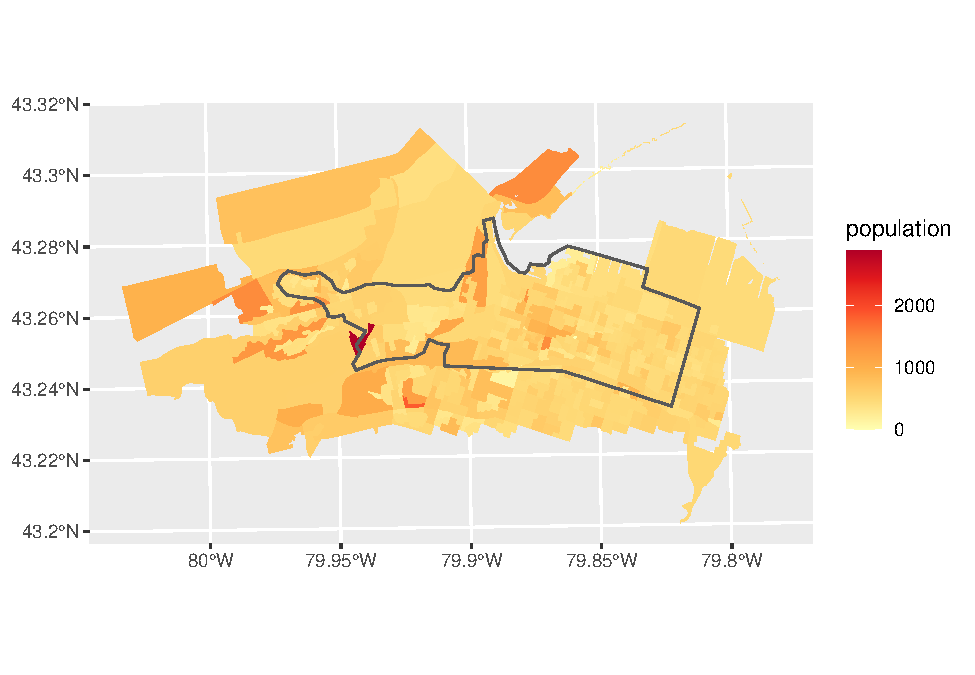
\includegraphics{00-Data-Processing-Example_files/figure-latex/unnamed-chunk-52-1.pdf}

Plot ``Green'' spaces:

\begin{Shaded}
\begin{Highlighting}[]
\KeywordTok{ggplot}\NormalTok{() }\OperatorTok{+}
\StringTok{  }\KeywordTok{geom_sf}\NormalTok{(}\DataTypeTok{data =}\NormalTok{ parks_sobi,}
          \DataTypeTok{fill =} \StringTok{"blue"}\NormalTok{) }\OperatorTok{+}
\StringTok{  }\KeywordTok{geom_sf}\NormalTok{(}\DataTypeTok{data =}\NormalTok{ cemeteries_sobi,}
          \DataTypeTok{fill =} \StringTok{"gray"}\NormalTok{) }\OperatorTok{+}
\StringTok{  }\KeywordTok{geom_sf}\NormalTok{(}\DataTypeTok{data =}\NormalTok{ esa_sobi,}
          \DataTypeTok{fill =} \StringTok{"green"}\NormalTok{) }\OperatorTok{+}
\StringTok{  }\KeywordTok{geom_sf}\NormalTok{(}\DataTypeTok{data =}\NormalTok{ golf_sobi,}
          \DataTypeTok{fill =} \StringTok{"lightskyblue"}\NormalTok{) }\OperatorTok{+}
\StringTok{  }\KeywordTok{geom_sf}\NormalTok{(}\DataTypeTok{data =}\NormalTok{ employment_sobi,}
          \DataTypeTok{fill =} \StringTok{"purple"}\NormalTok{) }\OperatorTok{+}
\StringTok{  }\KeywordTok{geom_sf}\NormalTok{(}\DataTypeTok{data =}\NormalTok{ railways_sobi,}
          \DataTypeTok{fill =} \StringTok{"wheat"}\NormalTok{) }\OperatorTok{+}
\StringTok{  }\KeywordTok{geom_sf}\NormalTok{(}\DataTypeTok{data =}\NormalTok{ parking_sobi,}
          \DataTypeTok{fill =} \StringTok{"lightpink"}\NormalTok{) }\OperatorTok{+}
\StringTok{  }\KeywordTok{geom_sf}\NormalTok{(}\DataTypeTok{data =}\NormalTok{ highways_sobi,}
          \DataTypeTok{fill =} \StringTok{"orange"}\NormalTok{) }\OperatorTok{+}
\StringTok{  }\KeywordTok{geom_sf}\NormalTok{(}\DataTypeTok{data =}\NormalTok{ schools_sobi,}
          \DataTypeTok{fill =} \StringTok{"red"}\NormalTok{) }\OperatorTok{+}
\StringTok{  }\KeywordTok{geom_sf}\NormalTok{(}\DataTypeTok{data =}\NormalTok{ religious_sobi,}
          \DataTypeTok{fill =} \StringTok{"pink"}\NormalTok{) }\OperatorTok{+}
\StringTok{  }\KeywordTok{geom_sf}\NormalTok{(}\DataTypeTok{data =}\NormalTok{ service_sobi,}
          \DataTypeTok{fill =} \StringTok{"yellow"}\NormalTok{) }\OperatorTok{+}
\StringTok{  }\KeywordTok{geom_sf}\NormalTok{(}\DataTypeTok{data =}\NormalTok{ recreation_sobi,}
          \DataTypeTok{fill =} \StringTok{"yellow"}\NormalTok{) }\OperatorTok{+}
\StringTok{  }\KeywordTok{geom_sf}\NormalTok{(}\DataTypeTok{data =}\NormalTok{ arenas_sobi,}
          \DataTypeTok{fill =} \StringTok{"yellow"}\NormalTok{) }\OperatorTok{+}
\StringTok{  }\KeywordTok{geom_sf}\NormalTok{(}\DataTypeTok{data =}\NormalTok{ ems_sobi,}
          \DataTypeTok{fill =} \StringTok{"yellow"}\NormalTok{) }\OperatorTok{+}
\StringTok{  }\KeywordTok{geom_sf}\NormalTok{(}\DataTypeTok{data =}\NormalTok{ ems_sobi,}
          \DataTypeTok{fill =} \StringTok{"yellow"}\NormalTok{) }\OperatorTok{+}
\StringTok{  }\KeywordTok{geom_sf}\NormalTok{(}\DataTypeTok{data =}\NormalTok{ fire_sobi,}
          \DataTypeTok{fill =} \StringTok{"yellow"}\NormalTok{) }\OperatorTok{+}
\StringTok{  }\KeywordTok{geom_sf}\NormalTok{(}\DataTypeTok{data =}\NormalTok{ police_sobi,}
          \DataTypeTok{fill =} \StringTok{"yellow"}\NormalTok{) }\OperatorTok{+}
\StringTok{  }\KeywordTok{geom_sf}\NormalTok{(}\DataTypeTok{data =}\NormalTok{ hospitals_sobi,}
          \DataTypeTok{fill =} \StringTok{"yellow"}\NormalTok{) }\OperatorTok{+}
\StringTok{  }\KeywordTok{geom_sf}\NormalTok{(}\DataTypeTok{data =}\NormalTok{ sobi_service,}
          \DataTypeTok{fill =} \OtherTok{NA}\NormalTok{,}
          \DataTypeTok{color =} \StringTok{"black"}\NormalTok{) }\OperatorTok{+}
\StringTok{  }\KeywordTok{geom_sf}\NormalTok{(}\DataTypeTok{data =}\NormalTok{ hamilton_da_sobi,}
          \DataTypeTok{fill =} \OtherTok{NA}\NormalTok{,}
          \DataTypeTok{color =} \StringTok{"gray"}\NormalTok{) }\OperatorTok{+}
\StringTok{  }\KeywordTok{scale_fill_distiller}\NormalTok{(}\DataTypeTok{palette =} \StringTok{"YlOrRd"}\NormalTok{, }\DataTypeTok{direction =} \DecValTok{1}\NormalTok{)}
\end{Highlighting}
\end{Shaded}

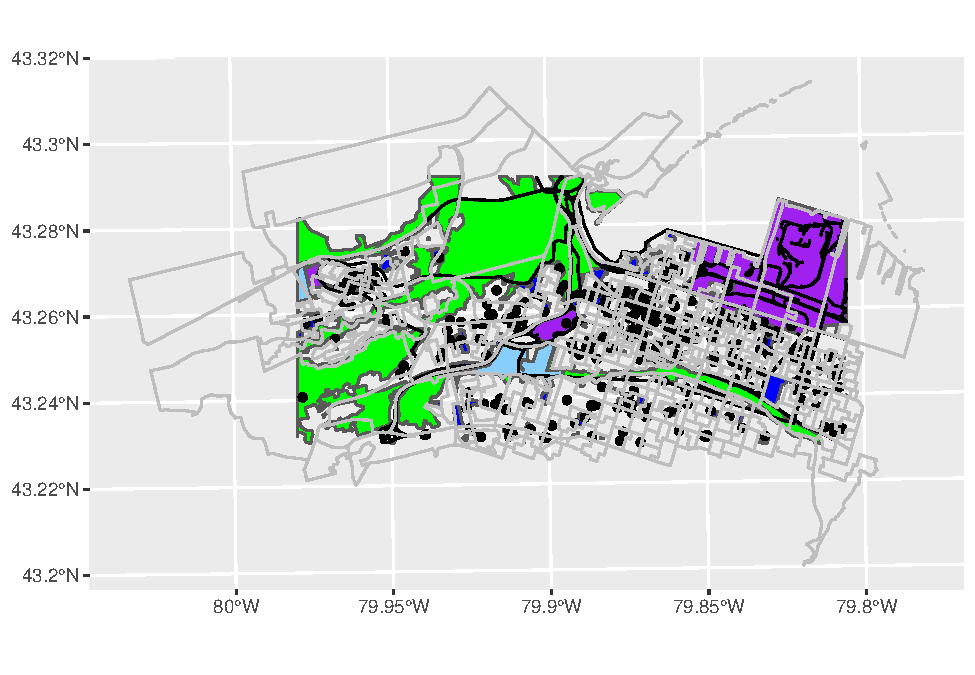
\includegraphics{00-Data-Processing-Example_files/figure-latex/unnamed-chunk-53-1.pdf}

\hypertarget{prepare-geographical-data-for-interpolation}{%
\subsubsection{Prepare geographical data for
interpolation}\label{prepare-geographical-data-for-interpolation}}

Union of the ``green space'' features:

\begin{Shaded}
\begin{Highlighting}[]
\NormalTok{parks_sobi <-}\StringTok{ }\KeywordTok{st_combine}\NormalTok{(parks_sobi)}
\NormalTok{cemeteries_sobi <-}\StringTok{ }\KeywordTok{st_combine}\NormalTok{(cemeteries_sobi)}
\NormalTok{esa_sobi <-}\StringTok{ }\KeywordTok{st_combine}\NormalTok{(esa_sobi)}
\NormalTok{golf_sobi <-}\StringTok{ }\KeywordTok{st_combine}\NormalTok{(golf_sobi)}
\NormalTok{employment_sobi <-}\StringTok{ }\KeywordTok{st_combine}\NormalTok{(employment_sobi)}
\NormalTok{railways_sobi <-}\StringTok{ }\KeywordTok{st_combine}\NormalTok{(railways_sobi)}
\NormalTok{parking_sobi <-}\StringTok{ }\KeywordTok{st_combine}\NormalTok{(parking_sobi)}
\NormalTok{highways_sobi <-}\StringTok{ }\KeywordTok{st_combine}\NormalTok{(highways_sobi)}
\NormalTok{schools_sobi <-}\StringTok{ }\KeywordTok{st_combine}\NormalTok{(schools_sobi)}
\NormalTok{religious_sobi <-}\StringTok{ }\KeywordTok{st_combine}\NormalTok{(religious_sobi)}
\NormalTok{service_sobi <-}\StringTok{ }\KeywordTok{st_combine}\NormalTok{(service_sobi)}
\NormalTok{recreation_sobi <-}\StringTok{ }\KeywordTok{st_combine}\NormalTok{(recreation_sobi)}
\NormalTok{arenas_sobi <-}\StringTok{ }\KeywordTok{st_combine}\NormalTok{(arenas_sobi)}
\NormalTok{ems_sobi <-}\StringTok{ }\KeywordTok{st_combine}\NormalTok{(ems_sobi)}
\NormalTok{fire_sobi <-}\StringTok{ }\KeywordTok{st_combine}\NormalTok{(fire_sobi)}
\NormalTok{police_sobi <-}\StringTok{ }\KeywordTok{st_combine}\NormalTok{(police_sobi)}
\NormalTok{hospitals_sobi <-}\StringTok{ }\KeywordTok{st_combine}\NormalTok{(hospitals_sobi)}
\end{Highlighting}
\end{Shaded}

Check that the topology is valid:

\begin{Shaded}
\begin{Highlighting}[]
\KeywordTok{st_is_valid}\NormalTok{(parks_sobi)}
\end{Highlighting}
\end{Shaded}

\begin{verbatim}
## [1] FALSE
\end{verbatim}

\begin{Shaded}
\begin{Highlighting}[]
\KeywordTok{st_is_valid}\NormalTok{(cemeteries_sobi)}
\end{Highlighting}
\end{Shaded}

\begin{verbatim}
## [1] TRUE
\end{verbatim}

\begin{Shaded}
\begin{Highlighting}[]
\KeywordTok{st_is_valid}\NormalTok{(esa_sobi)}
\end{Highlighting}
\end{Shaded}

\begin{verbatim}
## [1] FALSE
\end{verbatim}

\begin{Shaded}
\begin{Highlighting}[]
\KeywordTok{st_is_valid}\NormalTok{(golf_sobi)}
\end{Highlighting}
\end{Shaded}

\begin{verbatim}
## [1] TRUE
\end{verbatim}

\begin{Shaded}
\begin{Highlighting}[]
\KeywordTok{st_is_valid}\NormalTok{(employment_sobi)}
\end{Highlighting}
\end{Shaded}

\begin{verbatim}
## [1] TRUE
\end{verbatim}

\begin{Shaded}
\begin{Highlighting}[]
\KeywordTok{st_is_valid}\NormalTok{(railways_sobi)}
\end{Highlighting}
\end{Shaded}

\begin{verbatim}
## [1] TRUE
\end{verbatim}

\begin{Shaded}
\begin{Highlighting}[]
\KeywordTok{st_is_valid}\NormalTok{(parking_sobi)}
\end{Highlighting}
\end{Shaded}

\begin{verbatim}
## [1] FALSE
\end{verbatim}

\begin{Shaded}
\begin{Highlighting}[]
\KeywordTok{st_is_valid}\NormalTok{(highways_sobi)}
\end{Highlighting}
\end{Shaded}

\begin{verbatim}
## [1] TRUE
\end{verbatim}

\begin{Shaded}
\begin{Highlighting}[]
\KeywordTok{st_is_valid}\NormalTok{(schools_sobi)}
\end{Highlighting}
\end{Shaded}

\begin{verbatim}
## [1] TRUE
\end{verbatim}

\begin{Shaded}
\begin{Highlighting}[]
\KeywordTok{st_is_valid}\NormalTok{(religious_sobi)}
\end{Highlighting}
\end{Shaded}

\begin{verbatim}
## [1] TRUE
\end{verbatim}

\begin{Shaded}
\begin{Highlighting}[]
\KeywordTok{st_is_valid}\NormalTok{(service_sobi)}
\end{Highlighting}
\end{Shaded}

\begin{verbatim}
## [1] TRUE
\end{verbatim}

\begin{Shaded}
\begin{Highlighting}[]
\KeywordTok{st_is_valid}\NormalTok{(recreation_sobi)}
\end{Highlighting}
\end{Shaded}

\begin{verbatim}
## [1] TRUE
\end{verbatim}

\begin{Shaded}
\begin{Highlighting}[]
\KeywordTok{st_is_valid}\NormalTok{(arenas_sobi)}
\end{Highlighting}
\end{Shaded}

\begin{verbatim}
## [1] TRUE
\end{verbatim}

\begin{Shaded}
\begin{Highlighting}[]
\KeywordTok{st_is_valid}\NormalTok{(ems_sobi)}
\end{Highlighting}
\end{Shaded}

\begin{verbatim}
## [1] TRUE
\end{verbatim}

\begin{Shaded}
\begin{Highlighting}[]
\KeywordTok{st_is_valid}\NormalTok{(fire_sobi)}
\end{Highlighting}
\end{Shaded}

\begin{verbatim}
## [1] TRUE
\end{verbatim}

\begin{Shaded}
\begin{Highlighting}[]
\KeywordTok{st_is_valid}\NormalTok{(police_sobi)}
\end{Highlighting}
\end{Shaded}

\begin{verbatim}
## [1] TRUE
\end{verbatim}

\begin{Shaded}
\begin{Highlighting}[]
\KeywordTok{st_is_valid}\NormalTok{(hospitals_sobi)}
\end{Highlighting}
\end{Shaded}

\begin{verbatim}
## [1] TRUE
\end{verbatim}

Make valid:

\begin{Shaded}
\begin{Highlighting}[]
\NormalTok{parks_sobi <-}\StringTok{ }\KeywordTok{st_make_valid}\NormalTok{(parks_sobi)}
\NormalTok{esa_sobi <-}\StringTok{ }\KeywordTok{st_make_valid}\NormalTok{(esa_sobi)}
\NormalTok{parking_sobi <-}\StringTok{ }\KeywordTok{st_make_valid}\NormalTok{(parking_sobi)}
\end{Highlighting}
\end{Shaded}

\hypertarget{remove-all-features-that-are-not-population-from-the-das}{%
\subsubsection{Remove all features that are not population from the
DAs}\label{remove-all-features-that-are-not-population-from-the-das}}

Remove the parks from the DAs (use \texttt{st\_difference()}):

\begin{Shaded}
\begin{Highlighting}[]
\NormalTok{hamilton_da_sobi_clean <-}\StringTok{ }\KeywordTok{st_difference}\NormalTok{(hamilton_da_sobi, parks_sobi)}
\end{Highlighting}
\end{Shaded}

\begin{verbatim}
## Warning: attribute variables are assumed to be spatially constant throughout all
## geometries
\end{verbatim}

Remove the cemeteries from the DAs (use \texttt{st\_difference()}):

\begin{Shaded}
\begin{Highlighting}[]
\NormalTok{hamilton_da_sobi_clean <-}\StringTok{ }\KeywordTok{st_difference}\NormalTok{(hamilton_da_sobi_clean, cemeteries_sobi)}
\end{Highlighting}
\end{Shaded}

\begin{verbatim}
## Warning: attribute variables are assumed to be spatially constant throughout all
## geometries
\end{verbatim}

Remove environmentally sensitive areas from the DAs (use
\texttt{st\_difference()}):

\begin{Shaded}
\begin{Highlighting}[]
\NormalTok{hamilton_da_sobi_clean <-}\StringTok{ }\KeywordTok{st_difference}\NormalTok{(hamilton_da_sobi_clean, esa_sobi)}
\end{Highlighting}
\end{Shaded}

\begin{verbatim}
## Warning: attribute variables are assumed to be spatially constant throughout all
## geometries
\end{verbatim}

Remove golf courses from the DAs (use \texttt{st\_difference()}):

\begin{Shaded}
\begin{Highlighting}[]
\NormalTok{hamilton_da_sobi_clean <-}\StringTok{ }\KeywordTok{st_difference}\NormalTok{(hamilton_da_sobi_clean, golf_sobi)}
\end{Highlighting}
\end{Shaded}

\begin{verbatim}
## Warning: attribute variables are assumed to be spatially constant throughout all
## geometries
\end{verbatim}

Remove employment lands from the DAs (use \texttt{st\_difference()}):

\begin{Shaded}
\begin{Highlighting}[]
\NormalTok{hamilton_da_sobi_clean <-}\StringTok{ }\KeywordTok{st_difference}\NormalTok{(hamilton_da_sobi_clean, employment_sobi)}
\end{Highlighting}
\end{Shaded}

\begin{verbatim}
## Warning: attribute variables are assumed to be spatially constant throughout all
## geometries
\end{verbatim}

Remove railways from the DAs (use \texttt{st\_difference()}):

\begin{Shaded}
\begin{Highlighting}[]
\NormalTok{hamilton_da_sobi_clean <-}\StringTok{ }\KeywordTok{st_difference}\NormalTok{(hamilton_da_sobi_clean, railways_sobi)}
\end{Highlighting}
\end{Shaded}

\begin{verbatim}
## Warning: attribute variables are assumed to be spatially constant throughout all
## geometries
\end{verbatim}

Remove municipal parking lots from the DAs (use
\texttt{st\_difference()}):

\begin{Shaded}
\begin{Highlighting}[]
\NormalTok{hamilton_da_sobi_clean <-}\StringTok{ }\KeywordTok{st_difference}\NormalTok{(hamilton_da_sobi_clean, parking_sobi)}
\end{Highlighting}
\end{Shaded}

\begin{verbatim}
## Warning: attribute variables are assumed to be spatially constant throughout all
## geometries
\end{verbatim}

Remove provincial highways from the DAs (use \texttt{st\_difference()}):

\begin{Shaded}
\begin{Highlighting}[]
\NormalTok{hamilton_da_sobi_clean <-}\StringTok{ }\KeywordTok{st_difference}\NormalTok{(hamilton_da_sobi_clean, highways_sobi)}
\end{Highlighting}
\end{Shaded}

\begin{verbatim}
## Warning: attribute variables are assumed to be spatially constant throughout all
## geometries
\end{verbatim}

Remove educational institutions from the DAs (use
\texttt{st\_difference()}):

\begin{Shaded}
\begin{Highlighting}[]
\NormalTok{hamilton_da_sobi_clean <-}\StringTok{ }\KeywordTok{st_difference}\NormalTok{(hamilton_da_sobi_clean, schools_sobi)}
\end{Highlighting}
\end{Shaded}

\begin{verbatim}
## Warning: attribute variables are assumed to be spatially constant throughout all
## geometries
\end{verbatim}

Remove places of worship from the DAs (use \texttt{st\_difference()}):

\begin{Shaded}
\begin{Highlighting}[]
\NormalTok{hamilton_da_sobi_clean <-}\StringTok{ }\KeywordTok{st_difference}\NormalTok{(hamilton_da_sobi_clean, religious_sobi)}
\end{Highlighting}
\end{Shaded}

\begin{verbatim}
## Warning: attribute variables are assumed to be spatially constant throughout all
## geometries
\end{verbatim}

Remove municipal service centres from the DAs (use
\texttt{st\_difference()}):

\begin{Shaded}
\begin{Highlighting}[]
\NormalTok{hamilton_da_sobi_clean <-}\StringTok{ }\KeywordTok{st_difference}\NormalTok{(hamilton_da_sobi_clean, service_sobi)}
\end{Highlighting}
\end{Shaded}

\begin{verbatim}
## Warning: attribute variables are assumed to be spatially constant throughout all
## geometries
\end{verbatim}

Remove recreation and community centres from the DAs (use
\texttt{st\_difference()}):

\begin{Shaded}
\begin{Highlighting}[]
\NormalTok{hamilton_da_sobi_clean <-}\StringTok{ }\KeywordTok{st_difference}\NormalTok{(hamilton_da_sobi_clean, recreation_sobi)}
\end{Highlighting}
\end{Shaded}

\begin{verbatim}
## Warning: attribute variables are assumed to be spatially constant throughout all
## geometries
\end{verbatim}

Remove arenas from the DAs (use \texttt{st\_difference()}):

\begin{Shaded}
\begin{Highlighting}[]
\NormalTok{hamilton_da_sobi_clean <-}\StringTok{ }\KeywordTok{st_difference}\NormalTok{(hamilton_da_sobi_clean, arenas_sobi)}
\end{Highlighting}
\end{Shaded}

\begin{verbatim}
## Warning: attribute variables are assumed to be spatially constant throughout all
## geometries
\end{verbatim}

Remove EMS stations from the DAs (use \texttt{st\_difference()}):

\begin{Shaded}
\begin{Highlighting}[]
\NormalTok{hamilton_da_sobi_clean <-}\StringTok{ }\KeywordTok{st_difference}\NormalTok{(hamilton_da_sobi_clean, ems_sobi)}
\end{Highlighting}
\end{Shaded}

\begin{verbatim}
## Warning: attribute variables are assumed to be spatially constant throughout all
## geometries
\end{verbatim}

Remove fire stations from the DAs (use \texttt{st\_difference()}):

\begin{Shaded}
\begin{Highlighting}[]
\NormalTok{hamilton_da_sobi_clean <-}\StringTok{ }\KeywordTok{st_difference}\NormalTok{(hamilton_da_sobi_clean, fire_sobi)}
\end{Highlighting}
\end{Shaded}

\begin{verbatim}
## Warning: attribute variables are assumed to be spatially constant throughout all
## geometries
\end{verbatim}

Remove police stations from the DAs (use \texttt{st\_difference()}):

\begin{Shaded}
\begin{Highlighting}[]
\NormalTok{hamilton_da_sobi_clean <-}\StringTok{ }\KeywordTok{st_difference}\NormalTok{(hamilton_da_sobi_clean, police_sobi)}
\end{Highlighting}
\end{Shaded}

\begin{verbatim}
## Warning: attribute variables are assumed to be spatially constant throughout all
## geometries
\end{verbatim}

Remove hospitals from the DAs (use \texttt{st\_difference()}):

\begin{Shaded}
\begin{Highlighting}[]
\NormalTok{hamilton_da_sobi_clean <-}\StringTok{ }\KeywordTok{st_difference}\NormalTok{(hamilton_da_sobi_clean, hospitals_sobi)}
\end{Highlighting}
\end{Shaded}

\begin{verbatim}
## Warning: attribute variables are assumed to be spatially constant throughout all
## geometries
\end{verbatim}

Plot the new DAs (minus green) and compare to original DAs:

\begin{Shaded}
\begin{Highlighting}[]
\KeywordTok{ggplot}\NormalTok{() }\OperatorTok{+}
\StringTok{  }\KeywordTok{geom_sf}\NormalTok{(}\DataTypeTok{data =}\NormalTok{ hamilton_da_sobi_clean,}
          \DataTypeTok{color =} \OtherTok{NA}\NormalTok{,}
          \DataTypeTok{fill =} \StringTok{"blue"}\NormalTok{) }\OperatorTok{+}
\StringTok{  }\KeywordTok{geom_sf}\NormalTok{(}\DataTypeTok{data =}\NormalTok{ hamilton_da_sobi,}
          \DataTypeTok{fill =} \OtherTok{NA}\NormalTok{,}
          \DataTypeTok{color =} \StringTok{"black"}\NormalTok{)}
\end{Highlighting}
\end{Shaded}

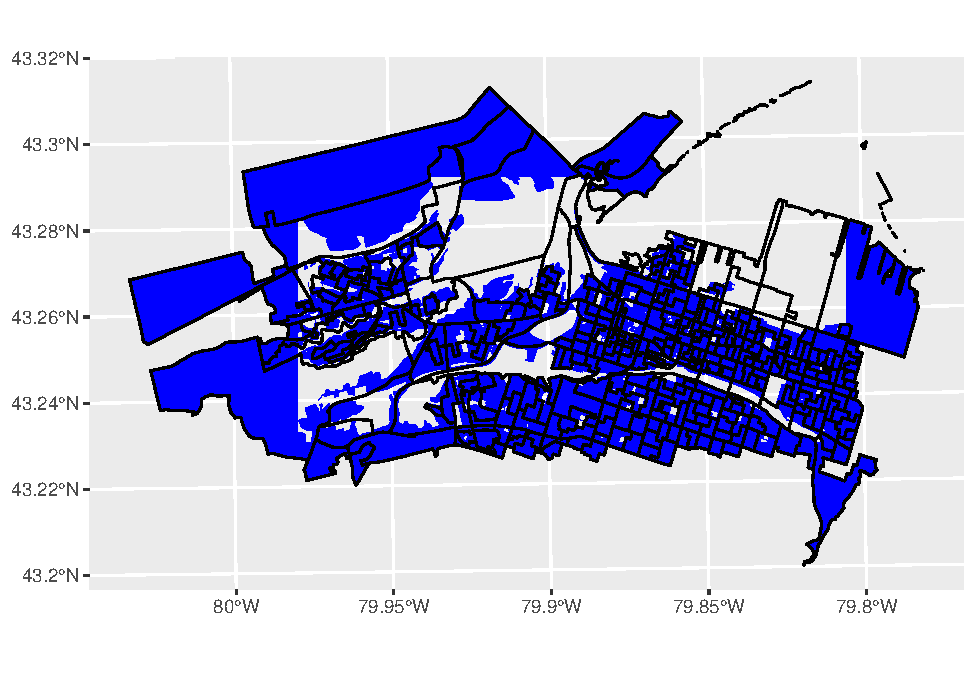
\includegraphics{00-Data-Processing-Example_files/figure-latex/unnamed-chunk-74-1.pdf}

\hypertarget{interpolate-population}{%
\subsection{Interpolate population}\label{interpolate-population}}

Pycnophylactic interpolation needs a \texttt{SpatialPolygonsDataFrame}
object. Convert the simple features object:

\begin{Shaded}
\begin{Highlighting}[]
\NormalTok{hamilton_da_sobi_clean.sp <-}\StringTok{ }\KeywordTok{as}\NormalTok{(hamilton_da_sobi_clean, }\StringTok{"Spatial"}\NormalTok{)}
\end{Highlighting}
\end{Shaded}

Extract the population from the spatial object:

\begin{Shaded}
\begin{Highlighting}[]
\NormalTok{pop <-}\StringTok{ }\NormalTok{hamilton_da_sobi_clean.sp}\OperatorTok{@}\NormalTok{data}\OperatorTok{$}\NormalTok{population}
\end{Highlighting}
\end{Shaded}

Pycnophylactic interpolation:

\begin{Shaded}
\begin{Highlighting}[]
\NormalTok{filter <-}\StringTok{ }\NormalTok{stats}\OperatorTok{::}\NormalTok{filter }\CommentTok{# Important! `filter()` should be from `stats`, not `dplyer`}
\NormalTok{interpolated_pop <-}\StringTok{ }\KeywordTok{pycno}\NormalTok{(}\DataTypeTok{x =}\NormalTok{ hamilton_da_sobi_clean.sp, }\DataTypeTok{pops =}\NormalTok{ pop, }\DataTypeTok{celldim =} \DecValTok{50}\NormalTok{)}
\end{Highlighting}
\end{Shaded}

\begin{verbatim}
## Warning in proj4string(x): CRS object has comment, which is lost in output
\end{verbatim}

\begin{verbatim}
## Maximum Change:     41.20295 - will stop at      0.11700
## Maximum Change:     15.53913 - will stop at      0.11700
## Maximum Change:     10.50693 - will stop at      0.11700
## Maximum Change:      6.89863 - will stop at      0.11700
## Maximum Change:      5.30048 - will stop at      0.11700
## Maximum Change:      3.68337 - will stop at      0.11700
## Maximum Change:      2.48480 - will stop at      0.11700
## Maximum Change:      2.01939 - will stop at      0.11700
## Maximum Change:      1.67714 - will stop at      0.11700
## Maximum Change:      1.42249 - will stop at      0.11700
## Maximum Change:      1.19921 - will stop at      0.11700
## Maximum Change:      1.02058 - will stop at      0.11700
## Maximum Change:      0.86826 - will stop at      0.11700
## Maximum Change:      0.74189 - will stop at      0.11700
## Maximum Change:      0.63467 - will stop at      0.11700
## Maximum Change:      0.54407 - will stop at      0.11700
## Maximum Change:      0.46724 - will stop at      0.11700
## Maximum Change:      0.40221 - will stop at      0.11700
## Maximum Change:      0.34688 - will stop at      0.11700
## Maximum Change:      0.29977 - will stop at      0.11700
## Maximum Change:      0.25950 - will stop at      0.11700
## Maximum Change:      0.22496 - will stop at      0.11700
## Maximum Change:      0.20150 - will stop at      0.11700
## Maximum Change:      0.18438 - will stop at      0.11700
## Maximum Change:      0.16802 - will stop at      0.11700
## Maximum Change:      0.15292 - will stop at      0.11700
## Maximum Change:      0.13920 - will stop at      0.11700
## Maximum Change:      0.12700 - will stop at      0.11700
## Maximum Change:      0.11602 - will stop at      0.11700
\end{verbatim}

\begin{verbatim}
## Warning in proj4string(x): CRS object has comment, which is lost in output
\end{verbatim}

Convert to pixels and then simple features:

\begin{Shaded}
\begin{Highlighting}[]
\NormalTok{interpolated_pop.pix <-}\StringTok{ }\KeywordTok{as}\NormalTok{(interpolated_pop, }\StringTok{"SpatialPixelsDataFrame"}\NormalTok{)}
\NormalTok{interpolated_pop <-}\StringTok{ }\KeywordTok{data.frame}\NormalTok{(}\DataTypeTok{population =}\NormalTok{ interpolated_pop.pix}\OperatorTok{$}\NormalTok{dens, }
                               \DataTypeTok{x =}\NormalTok{ interpolated_pop.pix}\OperatorTok{@}\NormalTok{coords[,}\DecValTok{1}\NormalTok{],}
                               \DataTypeTok{y =}\NormalTok{ interpolated_pop.pix}\OperatorTok{@}\NormalTok{coords[,}\DecValTok{2}\NormalTok{]) }\OperatorTok
\StringTok{  }\KeywordTok{st_as_sf}\NormalTok{(}\DataTypeTok{coords =} \KeywordTok{c}\NormalTok{(}\StringTok{"x"}\NormalTok{, }\StringTok{"y"}\NormalTok{),}
           \DataTypeTok{crs =} \KeywordTok{st_crs}\NormalTok{(hamilton_da_sobi))}
\end{Highlighting}
\end{Shaded}

Check the population totals:

\begin{Shaded}
\begin{Highlighting}[]
\KeywordTok{sum}\NormalTok{(hamilton_da_sobi_clean}\OperatorTok{$}\NormalTok{population)}
\end{Highlighting}
\end{Shaded}

\begin{verbatim}
## [1] 206539
\end{verbatim}

\begin{Shaded}
\begin{Highlighting}[]
\KeywordTok{sum}\NormalTok{(interpolated_pop}\OperatorTok{$}\NormalTok{population)}
\end{Highlighting}
\end{Shaded}

\begin{verbatim}
## [1] 206539
\end{verbatim}

Plot interpolated population:

\begin{Shaded}
\begin{Highlighting}[]
\KeywordTok{ggplot}\NormalTok{() }\OperatorTok{+}\StringTok{ }
\StringTok{  }\KeywordTok{geom_sf}\NormalTok{(}\DataTypeTok{data =}\NormalTok{ interpolated_pop,}
          \KeywordTok{aes}\NormalTok{(}\DataTypeTok{color =}\NormalTok{ population)) }\OperatorTok{+}
\StringTok{  }\KeywordTok{scale_color_distiller}\NormalTok{(}\DataTypeTok{palette =} \StringTok{"YlOrRd"}\NormalTok{, }
                        \DataTypeTok{direction =} \DecValTok{1}\NormalTok{) }\OperatorTok{+}
\StringTok{  }\KeywordTok{geom_sf}\NormalTok{(}\DataTypeTok{data =}\NormalTok{ hamilton_da_sobi,}
          \DataTypeTok{fill =} \OtherTok{NA}\NormalTok{,}
          \DataTypeTok{color =} \StringTok{"lightgray"}\NormalTok{) }\OperatorTok{+}\StringTok{ }
\StringTok{  }\KeywordTok{geom_sf}\NormalTok{(}\DataTypeTok{data =}\NormalTok{ sobi_service,}
          \DataTypeTok{fill =} \OtherTok{NA}\NormalTok{)}
\end{Highlighting}
\end{Shaded}

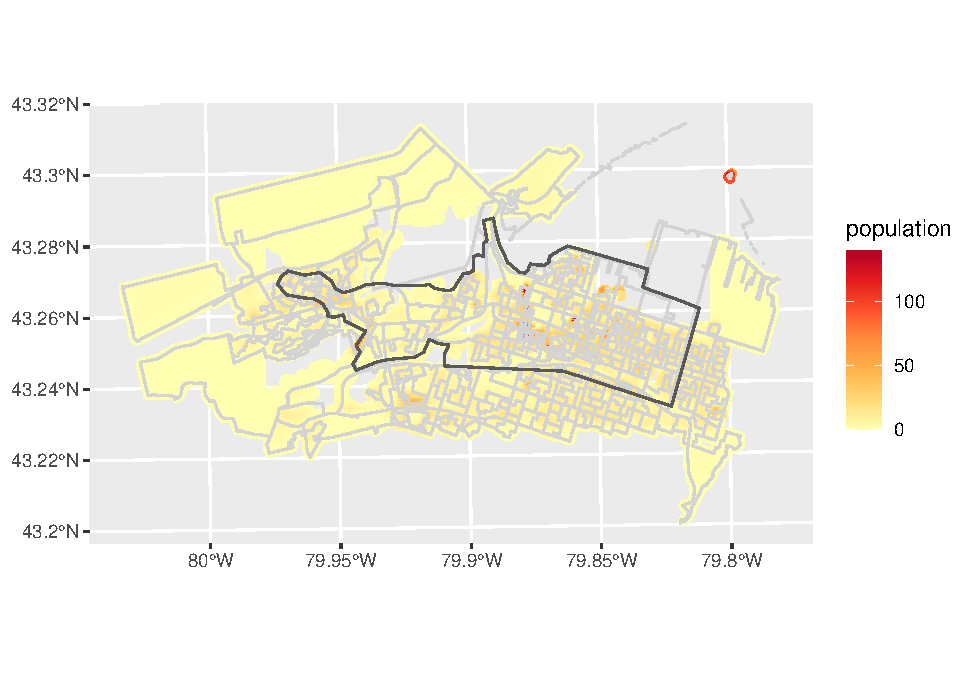
\includegraphics{00-Data-Processing-Example_files/figure-latex/unnamed-chunk-80-1.pdf}

\hypertarget{extract-population-in-service-area}{%
\subsection{Extract population in service
area}\label{extract-population-in-service-area}}

Extract population cells in the service area (and buffer)

\begin{Shaded}
\begin{Highlighting}[]
\NormalTok{interpolated_pop_clean <-}\StringTok{ }\NormalTok{interpolated_pop[sobi_service }\OperatorTok\StringTok{ }\KeywordTok{st_buffer}\NormalTok{(}\DecValTok{500}\NormalTok{),]}
\end{Highlighting}
\end{Shaded}

Note that some cells have population values of zero:

\begin{Shaded}
\begin{Highlighting}[]
\NormalTok{interpolated_pop_clean }\OperatorTok\StringTok{ }\NormalTok{dplyr}\OperatorTok{::}\KeywordTok{select}\NormalTok{(population) }\OperatorTok\StringTok{ }\KeywordTok{summary}\NormalTok{()}
\end{Highlighting}
\end{Shaded}

\begin{verbatim}
##    population               geometry    
##  Min.   :  0.000   POINT        :11902  
##  1st Qu.:  4.053   epsg:26917   :    0  
##  Median :  9.415   +proj=utm ...:    0  
##  Mean   : 11.564                        
##  3rd Qu.: 15.243                        
##  Max.   :140.184
\end{verbatim}

Filter all cells with non-zero population values:

\begin{Shaded}
\begin{Highlighting}[]
\NormalTok{interpolated_pop_clean <-}\StringTok{ }\NormalTok{interpolated_pop_clean }\OperatorTok
\StringTok{            }\NormalTok{dplyr}\OperatorTok{::}\KeywordTok{filter}\NormalTok{(population }\OperatorTok{>}\StringTok{ }\DecValTok{0}\NormalTok{)}
\end{Highlighting}
\end{Shaded}

Add identifier for the population cells:

\begin{Shaded}
\begin{Highlighting}[]
\NormalTok{interpolated_pop_clean <-}\StringTok{ }\NormalTok{interpolated_pop_clean }\OperatorTok
\StringTok{            }\KeywordTok{mutate}\NormalTok{(}\DataTypeTok{UID =} \DecValTok{1}\OperatorTok{:}\KeywordTok{n}\NormalTok{())}
\end{Highlighting}
\end{Shaded}

Plot interpolated population again:

\begin{Shaded}
\begin{Highlighting}[]
\KeywordTok{ggplot}\NormalTok{() }\OperatorTok{+}\StringTok{ }
\StringTok{  }\KeywordTok{geom_sf}\NormalTok{(}\DataTypeTok{data =}\NormalTok{ interpolated_pop_clean,}
          \KeywordTok{aes}\NormalTok{(}\DataTypeTok{color =}\NormalTok{ population)) }\OperatorTok{+}
\StringTok{  }\KeywordTok{geom_sf}\NormalTok{(}\DataTypeTok{data =}\NormalTok{ sobi_service,}
          \DataTypeTok{fill =} \OtherTok{NA}\NormalTok{) }\OperatorTok{+}
\StringTok{  }\KeywordTok{scale_color_distiller}\NormalTok{(}\DataTypeTok{palette =} \StringTok{"YlOrRd"}\NormalTok{, }
                        \DataTypeTok{direction =} \DecValTok{1}\NormalTok{)}
\end{Highlighting}
\end{Shaded}

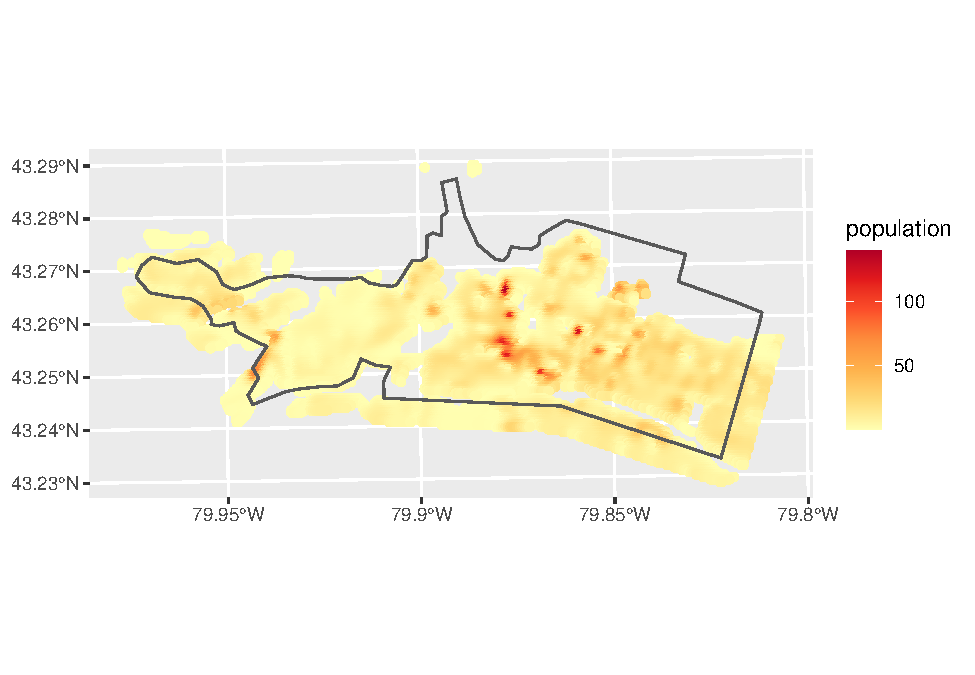
\includegraphics{00-Data-Processing-Example_files/figure-latex/unnamed-chunk-85-1.pdf}

\hypertarget{bikeshare-system}{%
\subsection{Bikeshare system}\label{bikeshare-system}}

Read Sobi hubs:

\begin{Shaded}
\begin{Highlighting}[]
\NormalTok{sobi_hubs <-}\StringTok{ }\KeywordTok{st_read}\NormalTok{(}\StringTok{"SoBi_Hubs.shp"}\NormalTok{)}
\end{Highlighting}
\end{Shaded}

\begin{verbatim}
## Reading layer `SoBi_Hubs' from data source `C:\Users\desjae\Documents\GitHub\Accessibility-Sobi-Hamilton\examples\SoBi_Hubs.shp' using driver `ESRI Shapefile'
## Simple feature collection with 134 features and 11 fields
## geometry type:  POINT
## dimension:      XY
## bbox:           xmin: 584909.4 ymin: 4788377 xmax: 600125.2 ymax: 4792103
## projected CRS:  NAD83 / UTM zone 17N
\end{verbatim}

Plot interpolated population and SoBi hubs:

\begin{Shaded}
\begin{Highlighting}[]
\KeywordTok{ggplot}\NormalTok{() }\OperatorTok{+}\StringTok{ }
\StringTok{  }\KeywordTok{geom_sf}\NormalTok{(}\DataTypeTok{data =}\NormalTok{ interpolated_pop_clean,}
          \KeywordTok{aes}\NormalTok{(}\DataTypeTok{color =}\NormalTok{ population)) }\OperatorTok{+}
\StringTok{  }\KeywordTok{geom_sf}\NormalTok{(}\DataTypeTok{data =}\NormalTok{ sobi_service,}
          \DataTypeTok{fill =} \OtherTok{NA}\NormalTok{) }\OperatorTok{+}
\StringTok{  }\KeywordTok{geom_sf}\NormalTok{(}\DataTypeTok{data =}\NormalTok{ sobi_hubs) }\OperatorTok{+}
\StringTok{  }\KeywordTok{scale_color_distiller}\NormalTok{(}\DataTypeTok{palette =} \StringTok{"YlOrRd"}\NormalTok{, }
                        \DataTypeTok{direction =} \DecValTok{1}\NormalTok{)}
\end{Highlighting}
\end{Shaded}

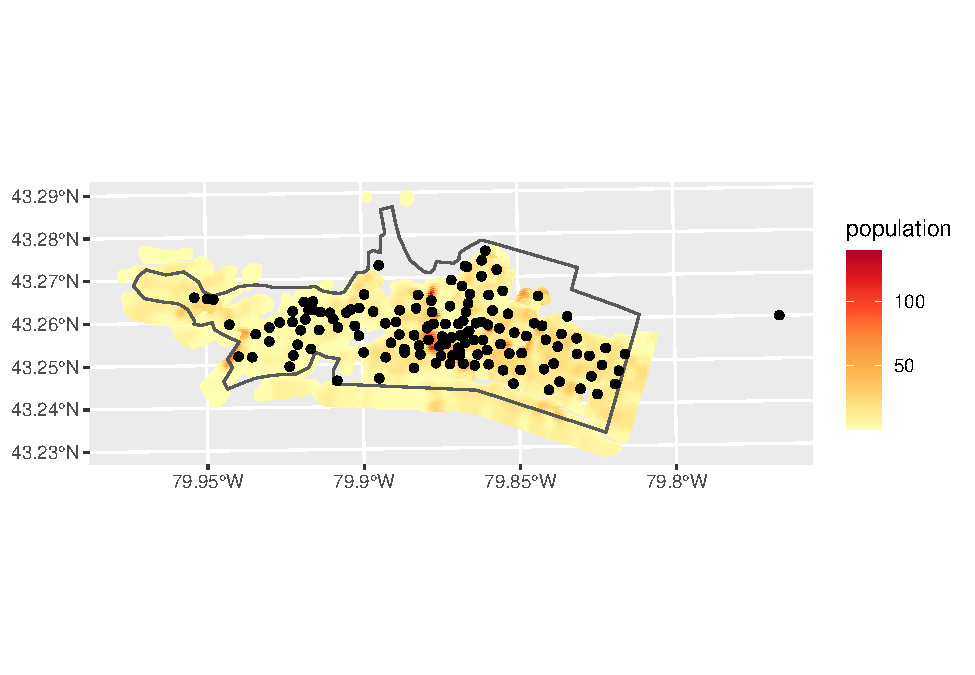
\includegraphics{00-Data-Processing-Example_files/figure-latex/unnamed-chunk-87-1.pdf}

Remove SoBi hub on beach:

\begin{Shaded}
\begin{Highlighting}[]
\NormalTok{sobi_hubs <-}\StringTok{ }\NormalTok{sobi_hubs }\OperatorTok
\StringTok{  }\NormalTok{dplyr}\OperatorTok{::}\KeywordTok{filter}\NormalTok{(NAME }\OperatorTok{!=}\StringTok{ "Van Wagners"}\NormalTok{)}
\end{Highlighting}
\end{Shaded}

Plot again:

\begin{Shaded}
\begin{Highlighting}[]
\KeywordTok{ggplot}\NormalTok{() }\OperatorTok{+}\StringTok{ }
\StringTok{  }\KeywordTok{geom_sf}\NormalTok{(}\DataTypeTok{data =}\NormalTok{ interpolated_pop_clean,}
          \KeywordTok{aes}\NormalTok{(}\DataTypeTok{color =}\NormalTok{ population)) }\OperatorTok{+}
\StringTok{  }\KeywordTok{geom_sf}\NormalTok{(}\DataTypeTok{data =}\NormalTok{ sobi_service,}
          \DataTypeTok{fill =} \OtherTok{NA}\NormalTok{) }\OperatorTok{+}
\StringTok{  }\KeywordTok{geom_sf}\NormalTok{(}\DataTypeTok{data =}\NormalTok{ sobi_hubs,}
          \KeywordTok{aes}\NormalTok{(}\DataTypeTok{size =}\NormalTok{ RACKS_AMOU)) }\OperatorTok{+}
\StringTok{  }\KeywordTok{scale_color_distiller}\NormalTok{(}\DataTypeTok{palette =} \StringTok{"YlOrRd"}\NormalTok{, }
                        \DataTypeTok{direction =} \DecValTok{1}\NormalTok{) }\OperatorTok{+}
\StringTok{  }\KeywordTok{scale_size}\NormalTok{(}\DataTypeTok{range =} \KeywordTok{c}\NormalTok{(}\DecValTok{1}\NormalTok{, }\DecValTok{4}\NormalTok{))}
\end{Highlighting}
\end{Shaded}

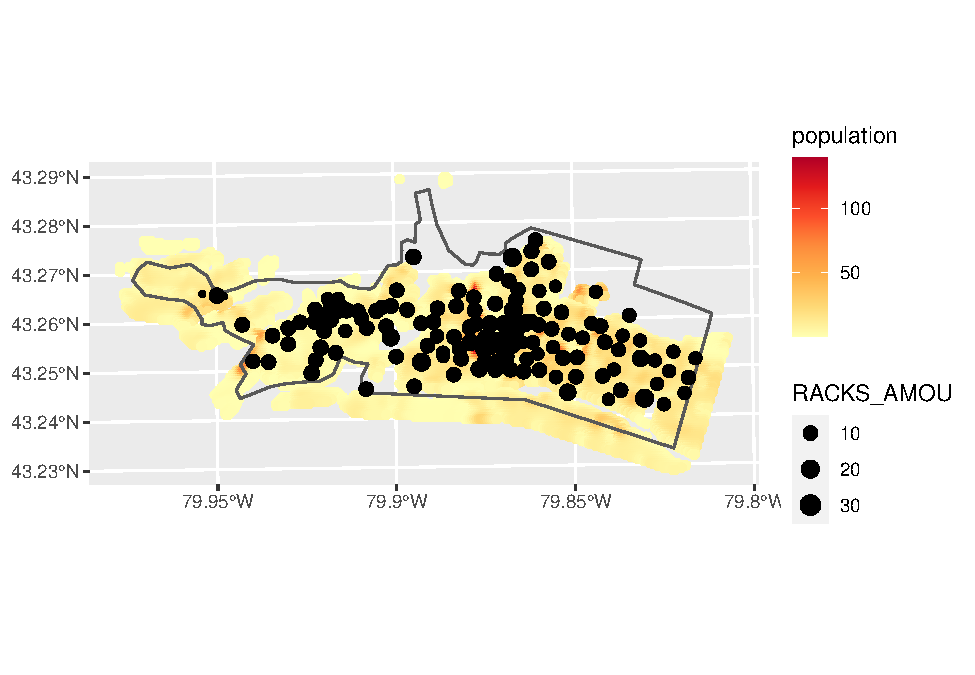
\includegraphics{00-Data-Processing-Example_files/figure-latex/unnamed-chunk-89-1.pdf}

Remove ERI hubs that were implemented in 2018 to increase accessibility
for under-serviced and disadvantaged areas of the city. This reflects
the original state of the system without the equity stations:

\begin{Shaded}
\begin{Highlighting}[]
\NormalTok{sobi_hubs_original <-}\StringTok{ }\NormalTok{sobi_hubs }\OperatorTok
\StringTok{  }\NormalTok{dplyr}\OperatorTok{::}\KeywordTok{filter}\NormalTok{(NAME }\OperatorTok{!=}\StringTok{ "Mars at Wentworth - ERI01"}\NormalTok{) }\OperatorTok
\StringTok{  }\NormalTok{dplyr}\OperatorTok{::}\KeywordTok{filter}\NormalTok{(NAME }\OperatorTok{!=}\StringTok{ "Sherman at Barton - ERI02"}\NormalTok{) }\OperatorTok
\StringTok{  }\NormalTok{dplyr}\OperatorTok{::}\KeywordTok{filter}\NormalTok{(NAME }\OperatorTok{!=}\StringTok{ "Barton at Lottridge - ERI03"}\NormalTok{) }\OperatorTok
\StringTok{  }\NormalTok{dplyr}\OperatorTok{::}\KeywordTok{filter}\NormalTok{(NAME }\OperatorTok{!=}\StringTok{ "Barton and Belview - ERI05"}\NormalTok{) }\OperatorTok
\StringTok{  }\NormalTok{dplyr}\OperatorTok{::}\KeywordTok{filter}\NormalTok{(NAME }\OperatorTok{!=}\StringTok{ "Barton at Ottawa - ERI06"}\NormalTok{) }\OperatorTok
\StringTok{  }\NormalTok{dplyr}\OperatorTok{::}\KeywordTok{filter}\NormalTok{(NAME }\OperatorTok{!=}\StringTok{ "Ottawa at Dunsmure - ERI07"}\NormalTok{) }\OperatorTok
\StringTok{  }\NormalTok{dplyr}\OperatorTok{::}\KeywordTok{filter}\NormalTok{(NAME }\OperatorTok{!=}\StringTok{ "Maple at Rothsay - ERI08"}\NormalTok{) }\OperatorTok
\StringTok{  }\NormalTok{dplyr}\OperatorTok{::}\KeywordTok{filter}\NormalTok{(NAME }\OperatorTok{!=}\StringTok{ "King at Dunsmure - ERI09"}\NormalTok{) }\OperatorTok
\StringTok{  }\NormalTok{dplyr}\OperatorTok{::}\KeywordTok{filter}\NormalTok{(NAME }\OperatorTok{!=}\StringTok{ "Dunsmure at Sherman - ERI10"}\NormalTok{) }\OperatorTok
\StringTok{  }\NormalTok{dplyr}\OperatorTok{::}\KeywordTok{filter}\NormalTok{(NAME }\OperatorTok{!=}\StringTok{ "Gage at Cannon - ERI11"}\NormalTok{) }\OperatorTok
\StringTok{  }\NormalTok{dplyr}\OperatorTok{::}\KeywordTok{filter}\NormalTok{(NAME }\OperatorTok{!=}\StringTok{ "Belview at Cannon - ERI12"}\NormalTok{) }\OperatorTok
\StringTok{  }\NormalTok{dplyr}\OperatorTok{::}\KeywordTok{filter}\NormalTok{(NAME }\OperatorTok{!=}\StringTok{ "Westinghouse at Barton - ERI13"}\NormalTok{)}
\end{Highlighting}
\end{Shaded}

Plot again:

\begin{Shaded}
\begin{Highlighting}[]
\KeywordTok{ggplot}\NormalTok{() }\OperatorTok{+}\StringTok{ }
\StringTok{  }\KeywordTok{geom_sf}\NormalTok{(}\DataTypeTok{data =}\NormalTok{ interpolated_pop_clean,}
          \KeywordTok{aes}\NormalTok{(}\DataTypeTok{color =}\NormalTok{ population)) }\OperatorTok{+}
\StringTok{  }\KeywordTok{geom_sf}\NormalTok{(}\DataTypeTok{data =}\NormalTok{ sobi_service,}
          \DataTypeTok{fill =} \OtherTok{NA}\NormalTok{) }\OperatorTok{+}
\StringTok{  }\KeywordTok{geom_sf}\NormalTok{(}\DataTypeTok{data =}\NormalTok{ sobi_hubs_original,}
          \KeywordTok{aes}\NormalTok{(}\DataTypeTok{size =}\NormalTok{ RACKS_AMOU)) }\OperatorTok{+}
\StringTok{  }\KeywordTok{scale_color_distiller}\NormalTok{(}\DataTypeTok{palette =} \StringTok{"YlOrRd"}\NormalTok{, }
                        \DataTypeTok{direction =} \DecValTok{1}\NormalTok{) }\OperatorTok{+}
\StringTok{  }\KeywordTok{scale_size}\NormalTok{(}\DataTypeTok{range =} \KeywordTok{c}\NormalTok{(}\DecValTok{1}\NormalTok{, }\DecValTok{4}\NormalTok{))}
\end{Highlighting}
\end{Shaded}

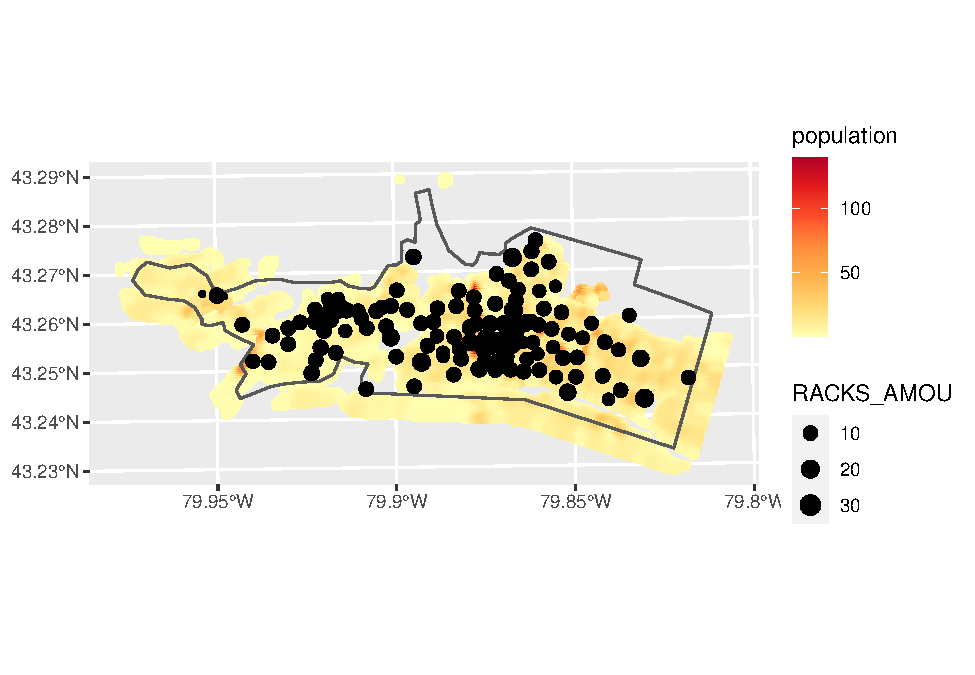
\includegraphics{00-Data-Processing-Example_files/figure-latex/unnamed-chunk-91-1.pdf}
After removing the twelve ERI hubs, there is much less coverage in the
east end of the service area. Again, the service area is the area where
a cyclist can use a SoBi bike. It makes sense then that ERI would want
to fill this gap in coverage because individuals who live in the east
end of the service area could theoretically use the bike share system
but may not live near a hub. For this reason, twelve hubs were added in
2018 to expand the system.

\hypertarget{routing-for-entire-system}{%
\subsection{Routing for entire system}\label{routing-for-entire-system}}

I used \href{https://download.bbbike.org/osm/bbbike/}{BBBike} to extract
OSM data for Hamilton - not the whole city, but enough to cover SoBI's
service area. The name of the file is
\texttt{planet\_-80.042,43.183\_-79.748,43.309.osm.pbf}. Copy to folder
\texttt{r5\_graph}.

Set Up R5 Routing. First define the path to where the graph is located:

Build the graph:

Prepare Input Data for \texttt{r5r}. The origins are the coordinates of
the population cells and the destinations the coordinates of the SoBi
hubs:

\begin{Shaded}
\begin{Highlighting}[]
\CommentTok{# save origin centroids in format expected by R5R (id, lon, lat)}
\NormalTok{origins_i <-}\StringTok{ }\KeywordTok{data.frame}\NormalTok{(}\DataTypeTok{UID =}\NormalTok{ interpolated_pop_clean}\OperatorTok{$}\NormalTok{UID, }
\NormalTok{              interpolated_pop_clean }\OperatorTok
\StringTok{                }\KeywordTok{st_transform}\NormalTok{(}\DataTypeTok{crs =} \DecValTok{4326}\NormalTok{) }\OperatorTok
\StringTok{                }\KeywordTok{st_coordinates}\NormalTok{()) }\OperatorTok
\StringTok{    }\KeywordTok{rename}\NormalTok{(}\DataTypeTok{lon =}\NormalTok{ X, }\DataTypeTok{lat =}\NormalTok{ Y, }\DataTypeTok{id =}\NormalTok{ UID) }\OperatorTok
\StringTok{    }\NormalTok{dplyr}\OperatorTok{::}\KeywordTok{select}\NormalTok{(id, lon, lat)}

\CommentTok{# now SoBi hubs}
\NormalTok{destinations_j <-}\StringTok{ }\KeywordTok{data.frame}\NormalTok{(}\DataTypeTok{OBJECTID =}\NormalTok{ sobi_hubs}\OperatorTok{$}\NormalTok{OBJECTID, }
\NormalTok{              sobi_hubs }\OperatorTok
\StringTok{                }\KeywordTok{st_transform}\NormalTok{(}\DataTypeTok{crs =} \DecValTok{4326}\NormalTok{) }\OperatorTok
\StringTok{                }\KeywordTok{st_coordinates}\NormalTok{()) }\OperatorTok
\StringTok{    }\KeywordTok{rename}\NormalTok{(}\DataTypeTok{lon =}\NormalTok{ X, }\DataTypeTok{lat =}\NormalTok{ Y, }\DataTypeTok{id =}\NormalTok{ OBJECTID) }\OperatorTok
\StringTok{    }\NormalTok{dplyr}\OperatorTok{::}\KeywordTok{select}\NormalTok{(id, lon, lat)}
\end{Highlighting}
\end{Shaded}

Calculate OD Matrix for Walking:

\hypertarget{extract-travel-time-matrix}{%
\subsection{Extract travel time
matrix}\label{extract-travel-time-matrix}}

Convert disk.frame to data frame:

\begin{Shaded}
\begin{Highlighting}[]
\NormalTok{ttm_walk <-}\StringTok{ }\KeywordTok{as.data.frame}\NormalTok{(ttm_walk.disk.frame) }\OperatorTok
\StringTok{  }\KeywordTok{transmute}\NormalTok{(}\DataTypeTok{UID =} \KeywordTok{as.numeric}\NormalTok{(fromId), }\DataTypeTok{OBJECTID =} \KeywordTok{as.numeric}\NormalTok{(toId), travel_time)}
\end{Highlighting}
\end{Shaded}

\hypertarget{routing-for-original-system-without-eri-hubs}{%
\subsection{Routing for original system without ERI
hubs}\label{routing-for-original-system-without-eri-hubs}}

Build the graph:

Prepare Input Data for \texttt{r5r}. The origins are the coordinates of
the population cells and the destinations the coordinates of the SoBi
hubs (minus the ERI hubs in the east end of the service area):

\begin{Shaded}
\begin{Highlighting}[]
\CommentTok{# save origin centroids in format expected by R5R (id, lon, lat)}
\NormalTok{origins_io <-}\StringTok{ }\KeywordTok{data.frame}\NormalTok{(}\DataTypeTok{UID =}\NormalTok{ interpolated_pop_clean}\OperatorTok{$}\NormalTok{UID, }
\NormalTok{              interpolated_pop_clean }\OperatorTok
\StringTok{                }\KeywordTok{st_transform}\NormalTok{(}\DataTypeTok{crs =} \DecValTok{4326}\NormalTok{) }\OperatorTok
\StringTok{                }\KeywordTok{st_coordinates}\NormalTok{()) }\OperatorTok
\StringTok{    }\KeywordTok{rename}\NormalTok{(}\DataTypeTok{lon =}\NormalTok{ X, }\DataTypeTok{lat =}\NormalTok{ Y, }\DataTypeTok{id =}\NormalTok{ UID) }\OperatorTok
\StringTok{    }\NormalTok{dplyr}\OperatorTok{::}\KeywordTok{select}\NormalTok{(id, lon, lat)}

\CommentTok{# now SoBi hubs}
\NormalTok{destinations_jo <-}\StringTok{ }\KeywordTok{data.frame}\NormalTok{(}\DataTypeTok{OBJECTID =}\NormalTok{ sobi_hubs_original}\OperatorTok{$}\NormalTok{OBJECTID, }
\NormalTok{              sobi_hubs_original }\OperatorTok
\StringTok{                }\KeywordTok{st_transform}\NormalTok{(}\DataTypeTok{crs =} \DecValTok{4326}\NormalTok{) }\OperatorTok
\StringTok{                }\KeywordTok{st_coordinates}\NormalTok{()) }\OperatorTok
\StringTok{    }\KeywordTok{rename}\NormalTok{(}\DataTypeTok{lon =}\NormalTok{ X, }\DataTypeTok{lat =}\NormalTok{ Y, }\DataTypeTok{id =}\NormalTok{ OBJECTID) }\OperatorTok
\StringTok{    }\NormalTok{dplyr}\OperatorTok{::}\KeywordTok{select}\NormalTok{(id, lon, lat)}
\end{Highlighting}
\end{Shaded}

Calculate OD Matrix for Walking:

\hypertarget{extract-travel-time-matrix-for-original-system}{%
\subsection{Extract travel time matrix for original
system}\label{extract-travel-time-matrix-for-original-system}}

Convert disk.frame to data frame:

\begin{Shaded}
\begin{Highlighting}[]
\NormalTok{ttm_walk_o <-}\StringTok{ }\KeywordTok{as.data.frame}\NormalTok{(ttm_walk_o.disk.frame) }\OperatorTok
\StringTok{  }\KeywordTok{transmute}\NormalTok{(}\DataTypeTok{UID =} \KeywordTok{as.numeric}\NormalTok{(fromId), }\DataTypeTok{OBJECTID =} \KeywordTok{as.numeric}\NormalTok{(toId), travel_time)}
\end{Highlighting}
\end{Shaded}

\hypertarget{save-data-to-disk}{%
\subsection{Save data to disk}\label{save-data-to-disk}}

Rename data frame:

\begin{Shaded}
\begin{Highlighting}[]
\NormalTok{population_sobi <-}\StringTok{ }\NormalTok{interpolated_pop_clean}
\end{Highlighting}
\end{Shaded}

Save data files:

\begin{Shaded}
\begin{Highlighting}[]
\KeywordTok{save}\NormalTok{(population_sobi, }\DataTypeTok{file =} \StringTok{"population_sobi.RData"}\NormalTok{)}
\KeywordTok{save}\NormalTok{(sobi_hubs, }\DataTypeTok{file =} \StringTok{"sobi_hubs.RData"}\NormalTok{)}
\KeywordTok{save}\NormalTok{(sobi_hubs_original, }\DataTypeTok{file =} \StringTok{"sobi_hubs_original.RData"}\NormalTok{)}
\KeywordTok{save}\NormalTok{(sobi_service, }\DataTypeTok{file =} \StringTok{"sobi_service.RData"}\NormalTok{)}
\KeywordTok{save}\NormalTok{(ttm_walk, }\DataTypeTok{file =} \StringTok{"ttm_walk.RData"}\NormalTok{)}
\KeywordTok{save}\NormalTok{(ttm_walk_o, }\DataTypeTok{file =} \StringTok{"ttm_walk_original.RData"}\NormalTok{)}
\end{Highlighting}
\end{Shaded}

\end{document}
